\documentclass[12pt]{report}
\usepackage[utf8]{inputenc}
% \usepackage[T1]{fontenc}
\usepackage[english]{babel}
\usepackage{fancyref}
% \usepackage{expex}
% \usepackage{hyphenat}
% \usepackage{tikz-qtree}
\usepackage{tikz}
\usepackage{tikz-dependency}
% \usetikzlibrary{calc}
% \usepackage[normalem]{ulem}
% \usepackage{amsmath}
\usepackage{amssymb} % has the \square for annotation illustrations
% \usepackage{amsthm}
\usepackage{ragged2e} % text-alignment but better
% \usepackage{floatrow}
\usepackage{hyperref}
% \usepackage{graphicx}
\usepackage{fancyhdr}
% \usepackage{fancyvrb}
% \usepackage{spverbatim}
% \usepackage[toc,page]{appendix}
% \usepackage{soul}
\usepackage[a4paper,width=140mm,top=25mm,bottom=25mm]{geometry}
% \usepackage{listings}
% \usepackage{multirow}
% \usepackage{footnote}
% \makesavenoteenv{tabular}
% \makesavenoteenv{table}
\usepackage{gb4e} % for linguistic examples
\usepackage{multicol}

\hypersetup{hidelinks}
\urlstyle{same}

% Fancy headers
\fancyhead{}
\fancyhead[L]{\footnotesize Dependency structure of English coordination: a surface-syntactic approach}
\fancyhead[R]{Chapter \thechapter }
\fancyfoot{}
\fancyfoot[C]{\thepage}

% For bibliography
% \usepackage[backend=biber,style=apa,sorting=nyt]{biblatex}
% \addbibresource{bibliography.bib}
\usepackage{natbib}
\bibliographystyle{apalike}

% Structure

\begin{document}

    \begin{titlepage}
	\begin{center}
		\vspace*{1.5cm}
		
		{\huge University of Warsaw}
		
		\vspace{0.1cm}
		{\Large Faculty of Philosophy}
		
		\vspace{3.5cm}
		
		{\Large Magdalena Borysiak} \\ Record book number: 446267
		
		\vspace{2cm}
		
		{\huge Dependency structure of English coordination: a surface-syntactic approach}
		
		
		\vspace{3cm}
		
		{\large Bachelor's thesis \\ in the field of Cognitive Science}
	\end{center}
	
	\vspace{2.5cm}
	
	\begin{flushright}
		The thesis was written under the supervision of \\
		prof. dr hab. Adam Przepiórkowski \\
		Faculty of Philosophy, University of Warsaw \\
		Institute of Computer Science, Polish Academy of Sciences	
	\end{flushright}
	
	\vspace{1.5cm}
	
	\begin{center}
		Warsaw, \monthyeardate\today
	\end{center}	
\end{titlepage}
    \pagestyle{empty}
    \section*{Summary}
    %\input{abstracts/abstract_EN.tex}
    \section*{Key words}
    %\input{abstracts/title&kws_EN.tex}
    \newpage
    \pagestyle{empty}
    \section*{Streszczenie}
    %\input{abstracts/abstract_PL.tex}
    \section*{Słowa kluczowe}
    %\input{abstracts/title&kws_PL.tex}
    
    % ToC %
    
    \tableofcontents
    
    % Chapters
    
    \pagestyle{fancy}
    \chapter{Introduction} \label{ch:introduction} % ten label jest do tego zeby robic reference btw
    The aim of this work is to expand on already existing research on the coordinate structures in the English language. A coordination is a structure which consists of multiple elements which serve the same function in the sentence and are often connected using a conjunction word. An example of a coordination from the Corpus of Contemporary American English \citep{coca} (COCA, henceforth) is given in (\ref{ex:govLeft}). There, the word \textsl{and} serves as the conjunction, \textsl{this} and \textsl{so many things} as the conjuncts.

\begin{exe}
    \ex
    \label{ex:govLeft} We're opposites \textsl{in} [[this] and [so many things]].
\end{exe}

This coordination is consistent with the observation that in English often the conjuncts on the left of a coordination are shorter than the ones on the right. According to \cite{prz:woz:23} however, the placement of the coordination's governor (the head of the whole structure, the word \textsl{in} in the example above) might have an influence on the way the coordination is structured: if the governor is on the left (as in (\ref{ex:govLeft})) or absent from the coordination altogether (as in (\ref{ex:govNone})), then the left conjunct will be shorter. That is not necessarily the case if the governor is on the right (as in (\ref{ex:govRight})).

\begin{exe}
    \ex\label{ex:govNone} [[She was right], but [he didn't want to say so]].
    \ex\label{ex:govRight} [[Cuban flags unfurled from windows] and [women wept]], Perez \textsl{says}.
\end{exe}

% longer version - explains more thoroughly DLM, but is that needed here?
% The proposed explanation for this comes from the fact that we often try to minimize the distance between connected constituents in a sentence. For example the sentence (3) tells us, that someone reported two events that happened: \textsl{Cuban flags unfurled from windows} and \textsl{women wept}. If that is the case, then those two event descriptions are connected to the word \textsl{says}. Now if we were to place those two descriptions the other way, by the time we got the the word \textsl{says}, we would have trouble recalling what was at the beginning of the sentence. Hence, according to some theories, we tend to shorten the dependencies in the sentences we produce.

% previous version:
%The proposed explanation for this is that Dependency Length Minimization can be observed here, which means that, when creating coordinate structures, we tend to try to minimize the distance between connected constituents. This was found to be the most likely explanation of the results and provided an argument for certain approaches to annotating the dependency structure of a coordination, namely the symmetrical ones. 

The Dependency Length Minimization effect is proposed as an explanation for this, which paired with the results of the research provides an argument for symmetric theories of coordination and against asymmetric ones. There were however some limitations to the research that needed to be addressed. The study was based on the Penn Treebank, a corpus already annotated with constituency structures. The presence of a manually approved syntactic annotation is a huge advantage for research like this, but unfortunately the corpus describes only a narrow fragment of the English language -- it is made up exclusively of the material from the Wall Street Journal and consists of 1.25M tokens, among which there were only 21,825 coordinations to analyse.

% next paragraph of the previous version:
%The research described above is based on the Penn Treebank, a corpus already annotated with constituency structures. Two advantages of such a resource are worth pointing out here: the presence of a manually approved syntactic annotation and the clear information about the exact length of a coordination's conjuncts. Unfortunately, the size of the corpus, as well as its lack of diversity cause the conducted research to describe only a narrow fragment of the English language -- it is made up exclusively of the material from the Wall Street Journal and consists of 1.25M tokens, among which there were only 21,825 coordinations to analyse.

A replication of those results using a different resource has already been attempted and described in an unpublished manuscript by \cite{pbg2023}. The results were similar, but more precise -- they supported not symmetric approaches to coordination in general, but specifically the multi-headed one. The corpus used there was COCA, which consists of over one billion words found in eight different genres ranging from academic to spoken. Unfortunately, it does not have any syntactic annotation that would immediately allow for data extraction and analysis similar to those in the study described above -- it had to be annotated automatically. Because of that, the quality of the data was significantly lower -- only 50.1\% of the coordinations included in the evaluation of data were parsed and extracted correctly. 

Issues with the data could possibly appear either at the parsing stage or at the extraction stage, and using Surface Syntactic Universal Dependencies (SUD) could help with both of those. According to \cite{tuo:prz:lac:21}, for some parsers (particularly the graph-based ones) the SUD annotation scheme might be easier to learn than Universal Dependencies -- the annotation scheme used in the replication study mentioned above. As for the issues at the extraction stage, the SUD scheme has some structural benefits, that can be used to create more accurate heuristics.

% another paragraph of the previous version:
%An example of a bigger and more diverse corpus is the Corpus of Contemporary American English. It consists of over one billion words found in eight different genres ranging from academic to spoken. One downside to this corpus is the absence of any syntactic annotation that would immediately allow for data extraction and analysis similar to those in the study described above. Automatic annotation should be therefore performed, for which the default choice is often the Universal Dependencies scheme \citep{nivre-etal-2020-universal} as seen for example in Stanza \citep{qi2020stanza}, Trankit \citep{nguyen2021trankit}, and COMBO \citep{klimaszewski-wroblewska-2021-combo-state}. However as \cite{prz:woz:23} mentioned, the UD annotation scheme would not be accurate for an analysis of coordination, as it cannot clearly distinguish between shared and private dependencies of a conjunct, thus making it problematic to measure its length -- information vital for this research. The Surface Syntactic Universal Dependencies scheme is an alternative worth considering for three reasons in particular. Firstly, the criteria for choosing dependency heads deployed in the SUD scheme generate syntactic trees without some of the ambiguities present in UD corpora. Secondly, more of those ambiguities can be resolved thanks to the explicitly marked shared dependencies in some coordinate structures. The final advantage of the SUD annotation here is that it can be easier to learn than the UD annotation for some parsers, particularly the graph-based ones \citep{tuo:prz:lac:21}. 

Work reported in this thesis is based on COCA annotated automatically using Stanza \citep{qi2020stanza}, a graph-based dependency parser, in accordance with the SUD annotation scheme. The structure of this thesis is the following: Chapter 2 describes in more detail some of the theoretical aspects mentioned in the current chapter -- this includes previous findings on coordinations in English, the Dependency Length Minimization effect and how it corresponds to different annotation schemes used in dependency treebanks, relevant differences between the UD and SUD annotation schemes and why the syntactic scheme seems to be more appropriate here. Chapter 3 describes how the corpus data was prepared for analysis -- from training the parser to extracting the information about coordinate structures. Chapter 4 presents the analysis of the data, which is discussed in Chapter 5. Finally Chapter 6 covers the limitations of this research. 
    \chapter{Theoretical background}
    \section{Dependency grammars}
% tesniere came up with a somewhat new (panini 600bc) way of creating a syntactic annotation. here are some basic ideas behind it, maybe why it could be useful
The first full-fledged theory of dependency grammar was proposed by \cite{tesniere-orig, tesniere}. One of the key ideas included in his work was that a sentence is not comprised solely of its words, but also of the connections between them -- dependencies. The connections he proposed were directed, therefore one of the two connected words is always a governor (head) and the other is a dependent. Another crucial element of Tesnière's approach was verb centrality -- the verb is the root of every sentence structure in dependency grammar. 

\begin{center}
\begin{exe}
	\ex\label{ex:tesniere}
    \begin{dependency}[theme = simple, baseline=-\the\dimexpr\fontdimen22\textfont2\relax]
    \begin{deptext}
        Alfred\& speaks\& slowly.\\
    \end{deptext}
    \depedge{2}{1}{}
    \depedge{2}{3}{}
    \end{dependency}
\end{exe}
\end{center}

% do i have to say it was used by tesniere? how do i say it?
Tesnière as an example used the sentence \textsl{Alfred speaks slowly}, for which a dependency tree is shown in (\ref{ex:tesniere}). It visualises the rules described above -- all of the words in a sentence are connected, those connections are directed and the verb is central to the whole structure. 

Dependency grammars have changed significantly since Tesnière's ideas were published. One example of such changes is the widespread usage of dependency labels, which describe the grammatical function that a word serves -- Tesnière differentiated only between actants and circumstants, which can be understood as obligatory dependencies of a verb, which complete its meaning, and optional dependencies, which are not necessary to complete the meaning of the verb. Different corpora have their own ideas for sets of dependency labels, for instance full annotation for (\ref{ex:tesniere}) could look similarly to (\ref{ex:tesniere today}), with the label \texttt{root} marking the central element of the sentence, \texttt{subj} marking the subject of the sentence and \texttt{mod} marking a modifier of the verb.

\begin{exe}
    \ex
    \label{ex:tesniere today}
    \begin{dependency}[theme = simple, baseline=-\the\dimexpr\fontdimen22\textfont2\relax]
    \begin{deptext}
        Alfred\&speaks\&slowly.\\
    \end{deptext}
    \deproot[edge height=5ex]{2}{root}
    \depedge{2}{1}{subj}
    \depedge{2}{3}{mod}
    \end{dependency}
\end{exe} 

Section \ref{sec:dlm} describes some specific phenomena that can be explained using dependency grammars. Section \ref{sec:coord annotations} presents some of the ideas for dependency annotation of coordinate structures that have been used in different corpora and Section \ref{sec:previous} describes the studies that were the basis for the present one. The last two sections of this chapter delve into more detail about two projects concerned with creating consistent dependency annotation schemes -- Universal Dependencies in Section \ref{sec:ud} and Surface-syntactic Universal Dependencies in Section \ref{sec:sud}. 

\section{Dependency length minimization}\label{sec:dlm}
% within this idea of dependencies in language, it was conceived that people while speaking try to minimise the dependencies in their utterances, so that it is easier to parse and understand, what they are trying to say. here are some studies about dlm and how this drive to shorten the dependencies may have affected grammar in some languages (hawkins94?)
% idk if it was within dependency grammars
% CITE TEMPERLEY 2018 SOMEWHERE HERE MAYBE
Familiarity with dependency grammars helps understand the principle of Dependency Length Minimization (henceforth DLM). It states that natural languages prefer shorter dependencies in their sentences. An example from \cite{hp83}, shown in (\ref{ex:dlm janitor}), illustrates this.

%is this really the best example? its very specific, because its about verb-particle constructions, maybe something more general would fit better
\begin{exe}
    \ex\label{ex:dlm janitor}
    \begin{xlist}
    \ex\label{ex:dlm janitor1}
    \begin{dependency}[theme = simple, segmented edge, baseline=-\the\dimexpr\fontdimen22\textfont2\relax]
        \begin{deptext}
        The\&janitor\&threw\&out\&the\&rickety\&and\&badly\&scratched\&chair.\\
        \end{deptext}
        \depedge{3}{4}{}
    \end{dependency}

    \ex\label{ex:dlm janitor2}
    \begin{dependency}[theme = simple, segmented edge, edge height = 4ex, baseline=-\the\dimexpr\fontdimen22\textfont2\relax]
        \begin{deptext}
        The\&janitor\&threw\&the\&rickety\&and\&badly\&scratched\&chair\&out.\\
        \end{deptext}
        \depedge{3}{10}{}
    \end{dependency}
    \end{xlist}
\end{exe}

The study has shown that speakers deem sentences similar to (\ref{ex:dlm janitor1}) more acceptable than the ones similar to (\ref{ex:dlm janitor2}).\footnote{In the study, it is actually found that it is not the distance between the verb and the particle that affects the acceptability of sentences like those, but the syntactic complexity of the phrases within that distance. However, according to \cite{wasow2002postverbal}, syntactic complexity as a measure of dependency length correlates with many others proposed, intervening words included.} Proposed explanations for this preference are based on language-processing constraints, which are usually said to be caused by working memory limitations. With longer dependencies, while reading or hearing a sentence, a person has to keep certain words in their working memory for a longer time. The longer the dependency, the harder the retrieval of the needed word from the working memory. Similar effects have been found in other studies, both psycholinguistic ones \citep{KING1991580, GIBSON19981} and those based on corpus research \citep{gildea-temperley-2007-optimizing, gildea-temperley-2010, futrell2020, dyer-2023}. 

% the idea of dlm in grammar and dlm in usage
The DLM effect has been observed both at the level of usage and at the level of grammar. The level of usage is visible in (\ref{ex:dlm janitor}) -- when there are multiple grammatical word orders available, people tend to choose those with shortest dependencies, because it makes the sentence easier to understand. As for DLM in grammar, an example taken from \cite[p.~20]{Hawkins-1994} is in (\ref{ex:hawkins-embed}). 
\begin{exe}
\ex\label{ex:hawkins-embed}
\begin{xlist}
	\ex[*] {Did _{S}[that John failed his exam] surprise Mary?}\label{ex:embedS}
	\ex[] {Did _{NP}[that fact] surprise Mary?}\label{ex:embedNP}
\end{xlist}
\end{exe}
Both of the sentences in (\ref{ex:hawkins-embed}) have a constituent embedded inside of them. In (\ref{ex:embedS}) that constituent is a subordinate clause \textsl{that John failed his exam}, whereas in (\ref{ex:embedNP}) the constituent is a noun phrase \textsl{that fact}. Subordinate clauses are usually longer than noun phrases, therefore dependencies in sentences with embedded clauses can be much longer. According to the DLM hypothesis, this makes the sentence more difficult to process and Hawkins argues that due to this processing difficulty sentences with clauses embedded this way are ungrammatical in English. Since noun phrases are usually shorter, sentences similar to (\ref{ex:embedNP}) are allowed. 

One of the earlier formulations of rules similar to DLM was made by \cite{behaghel}. He proposed two laws of word order:

\begin{itemize}
    \item[1.] That which belongs together mentally is placed close together.
    \item[2.] Of two sentence components, the shorter goes before the longer, when possible.
\end{itemize}

The first of these could be understood as DLM, while the other is a consequence of DLM in head-initial languages. Looking at how syntactic trees are usually shaped in a language allows for a judgement on the headedness or directionality of said language -- it can be head-initial if most dependencies are directed to right, or head-final if they are mostly directed to the left. English is an example of a head-initial language, therefore the second law proposed by Behaghel holds for English sentences. 

\section{Possible dependency structures of a coordination}\label{sec:coord annotations}
% coordination is a funny structure and there have been many ideas how to annotate them within the dependency approach to syntax. here are some ideas on how to do it, where they come from and maybe some rationale behind them

Different corpora choose different approaches to annotating the dependency structure of coordination. \cite{popel2013coordination} proposed a taxonomy of those, which consists of three families of annotation styles: Prague, Stanford and Moscow. \cite{prz:woz:23} add to those three a London family. All four of those families are described in more detail in the following subsections. Diagrams are used to better illustrate them, where:
\begin{itemize}
    \item $\odot$ is the governor of the coordination;
    \item each $\diamond$ symbolises a token, grouped together with a few others in a rectangle, forming a conjunct;
    \item $\square$ is the conjunction of the coordination.
\end{itemize}

Therefore the sentence \textsl{Mary and her younger sister laughed} using this set of symbols would look like in (\ref{ex:diagram}).

\begin{exe}
    \ex\label{ex:diagram}
\raisebox{-2.3ex}{
    \begin{minipage}{20em}
    \begin{dependency}
        \begin{deptext}
            Mary\&[.5cm]and\&[.5cm]her\&younger\&sister\&[.5cm]laughed\\
            \\
            $\diamond$\&$\square$\&\&$\diamond\diamond\diamond$\&\&$\odot$\\
        \end{deptext}
        \wordgroup{3}{1}{1}{}
        \wordgroup{3}{4}{4}{}
    \end{dependency}
    \end{minipage}
}
\end{exe}

% setting diagram heights and lengths
\newlength{\treeheight}
\newlength{\treewidth}
\settoheight{\treeheight}{
\begin{dependency}[theme = simple]
    \begin{deptext}
        $\diamond$\&$\diamond$\&$\diamond$\&$\diamond$\&$\diamond$\&$\square$\&$\diamond$\&$\diamond$\&$\odot$\\
    \end{deptext}
    \depedge{9}{1}{}
    \depedge{1}{7}{}
    \depedge{7}{6}{}
    \wordgroup{1}{1}{5}{}
    \wordgroup{1}{7}{8}{}
\end{dependency}
}
\settowidth{\treewidth}{
\begin{dependency}[theme = simple]
    \begin{deptext}
        $\odot$\&$\diamond$\&$\diamond$\&$\square$\&$\diamond$\&$\diamond$\&$\diamond$\&$\diamond$\&$\diamond$\&$\odot$\\
    \end{deptext}
    \wordgroup{1}{2}{3}{}
    \wordgroup{1}{5}{9}{}
\end{dependency}
}

In all of the diagrams in the current section it is assumed that the head of the conjunct is its first word. This assumption is justified, because the work presented here is based solely on the English language, which is mostly head-initial, therefore the diagrams presented here are more likely to be shaped as they are here than in any other way.

\subsection{Bouquet/Stanford}
The bouquet structure comes from the Stanford parser \citep{de-marneffe-etal-2006-generating}. Coordination with three conjuncts and a governor on the left would be annotated in the bouquet approach as shown in (\ref{ex:stanford}).

\begin{exe}
\ex\label{ex:stanford}
\begin{dependency}[theme = simple, baseline=-\the\dimexpr\fontdimen22\textfont2\relax]
        \begin{deptext}
        $\odot$\&$\diamond$\&$\diamond$\&$\diamond$\&,\&$\diamond$\&$\diamond$\&$\diamond$\&$\square$\&$\diamond$\&$\diamond$\&$\diamond$\\
            \end{deptext}
            \depedge{1}{2}{}
            \depedge{2}{6}{}
            \depedge{2}{10}{}
            \depedge{10}{9}{}
            \wordgroup{1}{2}{4}{c1}
            \wordgroup{1}{6}{8}{c2}
            \wordgroup{1}{10}{12}{c3}
        \end{dependency}
\end{exe}

In this approach there is a dependency connecting the governor of the coordination to the first conjunct, which is then connected to the heads of each conjunct, thus forming a bouquet. The conjunction is attached to the last conjunct in the structure. This structure is one of the asymmetrical ones, since it does not treat all conjuncts of the coordination equally -- it places emphasis on the first conjunct of a coordination by making it the head of every other conjunct. 

\vspace{-0.5\treeheight}

\begin{exe}
\ex\label{ex:stanford-all}
\raisebox{-0.5ex}{
\begin{minipage}[t]{2.5\treewidth}
\begin{xlist}

\begin{multicols}{2}

\ex
\begin{minipage}[b][\treeheight]{\treewidth}
\vfill
% gov on the left, shorter conj on the left
\begin{dependency}[theme = simple, baseline=-\the\dimexpr\fontdimen22\textfont2\relax]
    \begin{deptext}
        $\odot$\&$\diamond$\&$\diamond$\&$\square$\&$\diamond$\&$\diamond$\&$\diamond$\&$\diamond$\&$\diamond$\\
    \end{deptext}
    \depedge{1}{2}{}
    \depedge{2}{5}{}
    \depedge{5}{4}{}
    \wordgroup{1}{2}{3}{}
    \wordgroup{1}{5}{9}{}
\end{dependency}
\end{minipage}

\columnbreak

\ex
\begin{minipage}[b][\treeheight]{\treewidth}
% gov on the left, shorter conj on the right
\begin{dependency}[theme = simple, baseline=-\the\dimexpr\fontdimen22\textfont2\relax]
    \begin{deptext}
        $\odot$\&$\diamond$\&$\diamond$\&$\diamond$\&$\diamond$\&$\diamond$\&$\square$\&$\diamond$\&$\diamond$\\
    \end{deptext}
    \depedge{1}{2}{}
    \depedge{2}{8}{}
    \depedge{8}{7}{}
    \wordgroup{1}{2}{6}{}
    \wordgroup{1}{8}{9}{}
\end{dependency}
\end{minipage}
\end{multicols}

\begin{multicols}{2}

\ex
\begin{minipage}[b][\treeheight]{\treewidth}
\vfill
% gov absent, shorter conj on the left
\phantom{$\odot$}\hspace{\fontdimen4\font}
\begin{dependency}[theme = simple, baseline=-\the\dimexpr\fontdimen22\textfont2\relax]
    \begin{deptext}
        $\diamond$\&$\diamond$\&$\square$\&$\diamond$\&$\diamond$\&$\diamond$\&$\diamond$\&$\diamond$\\
    \end{deptext}
    \deproot[edge height=4ex]{1}{}
    \depedge{1}{4}{}
    \depedge{4}{3}{}
    \wordgroup{1}{1}{2}{}
    \wordgroup{1}{4}{8}{}
\end{dependency}
\end{minipage}

\columnbreak

\ex
\begin{minipage}[b][\treeheight]{\treewidth}
% gov absent, shorter conj on the right
\phantom{$\odot$}\hspace{\fontdimen4\font}
\begin{dependency}[theme = simple, baseline=-\the\dimexpr\fontdimen22\textfont2\relax]
    \begin{deptext}
        $\diamond$\&$\diamond$\&$\diamond$\&$\diamond$\&$\diamond$\&$\square$\&$\diamond$\&$\diamond$\\
    \end{deptext}
    \deproot[edge height=4ex]{1}{}
    \depedge{1}{7}{}
    \depedge{7}{6}{}
    \wordgroup{1}{1}{5}{}
    \wordgroup{1}{7}{8}{}
\end{dependency}
\end{minipage}
\end{multicols}

\begin{multicols}{2}

\ex
\begin{minipage}[b][\treeheight]{\treewidth}
% gov on the right, shorter conj on the left
\phantom{$\odot$}\hspace{\fontdimen4\font}
\begin{dependency}[theme = simple, baseline=-\the\dimexpr\fontdimen22\textfont2\relax]
    \begin{deptext}
        $\diamond$\&$\diamond$\&$\square$\&$\diamond$\&$\diamond$\&$\diamond$\&$\diamond$\&$\diamond$\&$\odot$\\
    \end{deptext}
    \depedge{9}{1}{}
    \depedge{1}{4}{}
    \depedge{4}{3}{}
    \wordgroup{1}{1}{2}{}
    \wordgroup{1}{4}{8}{}
\end{dependency}
\end{minipage}

\columnbreak

\ex
\begin{minipage}[b][\treeheight]{\treewidth}
% gov on the right, shorter conj on the right
\phantom{$\odot$}\hspace{\fontdimen4\font}
\begin{dependency}[theme = simple, baseline=-\the\dimexpr\fontdimen22\textfont2\relax]
    \begin{deptext}
        $\diamond$\&$\diamond$\&$\diamond$\&$\diamond$\&$\diamond$\&$\square$\&$\diamond$\&$\diamond$\&$\odot$\\
    \end{deptext}
    \depedge{9}{1}{}
    \depedge{1}{7}{}
    \depedge{7}{6}{}
    \wordgroup{1}{1}{5}{}
    \wordgroup{1}{7}{8}{}
\end{dependency}
\end{minipage}
\end{multicols}

\end{xlist}
\end{minipage}
}
\end{exe}

\vspace{0.5\treeheight}

The diagrams in (\ref{ex:stanford-all}) show the Stanford structure with different governor positions and conjunct placements. In (\ref{ex:stanford-all}a--b) the governor is on the left with the shorter conjunct on the left in (\ref{ex:stanford-all}a) and on the right in (\ref{ex:stanford-all}b). In those diagrams, two of the dependencies drawn have the same lenght in both cases, but the third one is visibly longer in (\ref{ex:stanford-all}b). This means that, according to the DLM principle, the structure in (\ref{ex:stanford-all}a) should be preferred over (\ref{ex:stanford-all}b), so coordinations with conjuncts of significantly different lengths should have the shorter conjunct on the left. 

Within the Stanford approach this is the case for every governor position. Diagrams (\ref{ex:stanford-all}c--d) show the structure of coordination when the governor is absent, with dependencies shorter in (\ref{ex:stanford-all}c) than in (\ref{ex:stanford-all}d), i.e., when the shorter conjunct is on the left. Diagrams (\ref{ex:stanford-all}e--f) show the structure when the governor is on the right, with dependencies shorter in (\ref{ex:stanford-all}e) than in (\ref{ex:stanford-all}f), also when the shorter conjunct is on the left. Therefore within this approach the position of the governor does not influence the preferred order of the conjuncts and the shorter conjunct should always be placed on the left. 

% to tu było ale nie wiem czy to ma sens tutaj:
% As the Universal Dependencies annotation scheme (described in Section \ref{sec:ud}) was based on the annotations produced by the Stanford Parser, the scheme now uses the Stanford style to annotate coordinations. 
\subsection{Chain/Moscow}
Another asymmetrical approach is the chain, or Moscow one. It is utilised in the Meaning-Text Theory proposed by \cite{melcuk-1988}. 

\begin{Center}
\begin{dependency}[theme = simple]
            \begin{deptext}
    $\odot$\&$\diamond$\&$\diamond$\&$\diamond$\&,\&$\diamond$\&$\diamond$\&$\diamond$\&$\square$\&$\diamond$\&$\diamond$\&$\diamond$\\
            \end{deptext}
            \depedge{1}{2}{}
            \depedge{2}{6}{}
            \depedge{6}{9}{}
            \depedge{9}{10}{}
            \wordgroup{1}{2}{4}{c1}
            \wordgroup{1}{6}{8}{c2}
            \wordgroup{1}{10}{12}{c3}
        \end{dependency}
\end{Center}

The structure is created by connecting the governor to the first conjunct of the coordination, then every other element of the coordination (including the conjunction) to the next one. As the dependency between the governor and the coordination is specifically between the governor and the first conjunct, the chain approach is another example of an asymmetrical annotation style. 

\begin{multicols}{2}
\begin{exe}
\ex
\label{ex:moscow-all}
\begin{xlist}
% gov on the left, shorter conj on the left
\ex
\begin{dependency}[theme = simple, baseline=-\the\dimexpr\fontdimen22\textfont2\relax]
    \begin{deptext}
        $\odot$\&$\diamond$\&$\diamond$\&$\square$\&$\diamond$\&$\diamond$\&$\diamond$\&$\diamond$\&$\diamond$\\
    \end{deptext}
    \depedge{1}{2}{}
    \depedge{2}{4}{}
    \depedge{4}{5}{}
    \wordgroup{1}{2}{3}{}
    \wordgroup{1}{5}{9}{}
\end{dependency}

\ex
% gov on the left, shorter conj on the right
\begin{dependency}[theme = simple, baseline=-\the\dimexpr\fontdimen22\textfont2\relax]
    \begin{deptext}
        $\odot$\&$\diamond$\&$\diamond$\&$\diamond$\&$\diamond$\&$\diamond$\&$\square$\&$\diamond$\&$\diamond$\\
    \end{deptext}
    \depedge{1}{2}{}
    \depedge{2}{7}{}
    \depedge{7}{8}{}
    \wordgroup{1}{2}{6}{}
    \wordgroup{1}{8}{9}{}
\end{dependency}

\ex
% gov absent, shorter conj on the left
\begin{dependency}[theme = simple, baseline=-\the\dimexpr\fontdimen22\textfont2\relax]
    \begin{deptext}
        $\diamond$\&$\diamond$\&$\square$\&$\diamond$\&$\diamond$\&$\diamond$\&$\diamond$\&$\diamond$\\
    \end{deptext}
    \deproot[edge height=4ex]{1}{}
    \depedge{1}{3}{}
    \depedge{3}{4}{}
    \wordgroup{1}{1}{2}{}
    \wordgroup{1}{4}{8}{}
\end{dependency}

\ex
% gov absent, shorter conj on the right
\begin{dependency}[theme = simple, baseline=-\the\dimexpr\fontdimen22\textfont2\relax]
    \begin{deptext}
        $\diamond$\&$\diamond$\&$\diamond$\&$\diamond$\&$\diamond$\&$\square$\&$\diamond$\&$\diamond$\\
    \end{deptext}
    \deproot[edge height=4ex]{1}{}
    \depedge{1}{6}{}
    \depedge{6}{7}{}
    \wordgroup{1}{1}{5}{}
    \wordgroup{1}{7}{8}{}
\end{dependency}

\ex
% gov on the right, shorter conj on the left
\begin{dependency}[theme = simple, baseline=-\the\dimexpr\fontdimen22\textfont2\relax]
    \begin{deptext}
        $\diamond$\&$\diamond$\&$\square$\&$\diamond$\&$\diamond$\&$\diamond$\&$\diamond$\&$\diamond$\&$\odot$\\
    \end{deptext}
    \depedge{9}{1}{}
    \depedge{1}{3}{}
    \depedge{3}{4}{}
    \wordgroup{1}{1}{2}{}
    \wordgroup{1}{4}{8}{}
\end{dependency}

\ex
% gov on the right, shorter conj on the right
\begin{dependency}[theme = simple, baseline=-\the\dimexpr\fontdimen22\textfont2\relax]
    \begin{deptext}
        $\diamond$\&$\diamond$\&$\diamond$\&$\diamond$\&$\diamond$\&$\square$\&$\diamond$\&$\diamond$\&$\odot$\\
    \end{deptext}
    \depedge{9}{1}{}
    \depedge{1}{6}{}
    \depedge{6}{7}{}
    \wordgroup{1}{1}{5}{}
    \wordgroup{1}{7}{8}{}

\end{dependency}
\end{xlist}
\end{exe}
\end{multicols}

The diagrams in (\ref{ex:moscow-all}) show that in this case, similarly to the bouquet approach, the placement of the shorter conjunct on the left would be preferred, assuming the DLM principle. The placement of the governor again does not seem to have an effect on the ordering. 

A variation of this annotation style is now used in the Surface-syntactic Universal Dependencies scheme (described in Section \ref{sec:sud}), which is based on the Universal Dependencies. The authors chose the Chain style instead of the Bouquet, as it minimizes the dependency lengths, which the authors wanted to be reflected in the syntactic structure. The difference between their style and the one shown in (\ref{ex:moscow-all}) is that the conjunction is not attached to the preceding conjunct, but to the next one. This annotation is illustrated in (\ref{ex:chain sud}). 

\begin{exe}
    \ex
    \label{ex:chain sud}
    \begin{Center}
    \begin{dependency}[theme = simple, baseline=-\the\dimexpr\fontdimen22\textfont2\relax]
            \begin{deptext}
    $\odot$\&$\diamond$\&$\diamond$\&$\diamond$\&,\&$\diamond$\&$\diamond$\&$\diamond$\&$\square$\&$\diamond$\&$\diamond$\&$\diamond$\\
            \end{deptext}
            \depedge{1}{2}{}
            \depedge{2}{6}{}
            \depedge{6}{10}{}
            \depedge{10}{9}{}
            \wordgroup{1}{2}{4}{c1}
            \wordgroup{1}{6}{8}{c2}
            \wordgroup{1}{10}{12}{c3}
        \end{dependency}
\end{Center}
\end{exe}
\subsection{Multi-headed/London}\label{sec:london}
The symmetrical approaches, as the name suggests, treat every conjunct in the coordination the same way. One of them is the multi-headed, or London approach, for which \cite{prz:woz:23} propose the name based on its appearance in Word Grammar, developed by \cite{hudson-1984, hudson-2010} at University College London.

\begin{exe}
\centering
\ex\label{ex:london}
\begin{dependency}[theme = simple, baseline=-\the\dimexpr\fontdimen22\textfont2\relax]
            \begin{deptext}
    $\odot$\&$\diamond$\&$\diamond$\&$\diamond$\&,\&$\diamond$\&$\diamond$\&$\diamond$\&$\square$\&$\diamond$\&$\diamond$\&$\diamond$\\
            \end{deptext}
            \depedge{1}{2}{}
            \depedge{1}{6}{}
            \depedge{1}{10}{}
            \depedge{10}{9}{}
            \wordgroup{1}{2}{4}{c1}
            \wordgroup{1}{6}{8}{c2}
            \wordgroup{1}{10}{12}{c3}
        \end{dependency}
\end{exe}

The symmetry of the approach comes from the fact that no conjunct is distinguished by being the only direct dependent of coordinations governor. Instead, all of the conjuncts have dependencies connecting them to the governor, and the conjunction is dependent on the last conjunct, similarly to the Stanford approach.

\vspace{-0.5\treeheight}

\begin{exe}
\ex\label{ex:london-all}
\raisebox{-0.5ex}{
\begin{minipage}[t]{2.5\treewidth}
\begin{xlist}

\begin{multicols}{2}

\ex
\begin{minipage}[b][\treeheight]{\treewidth}
\vfill
% gov on the left, shorter conj on the left
\begin{dependency}[theme = simple, baseline=-\the\dimexpr\fontdimen22\textfont2\relax]
    \begin{deptext}
        $\odot$\&$\diamond$\&$\diamond$\&$\square$\&$\diamond$\&$\diamond$\&$\diamond$\&$\diamond$\&$\diamond$\\
    \end{deptext}
    \depedge{1}{2}{}
    \depedge{1}{5}{}
    \depedge{5}{4}{}
    \wordgroup{1}{2}{3}{}
    \wordgroup{1}{5}{9}{}
\end{dependency}
\end{minipage}

\columnbreak

\ex
\begin{minipage}[b][\treeheight]{\treewidth}
% gov on the left, shorter conj on the right
\begin{dependency}[theme = simple, baseline=-\the\dimexpr\fontdimen22\textfont2\relax]
    \begin{deptext}
        $\odot$\&$\diamond$\&$\diamond$\&$\diamond$\&$\diamond$\&$\diamond$\&$\square$\&$\diamond$\&$\diamond$\\
    \end{deptext}
    \depedge{1}{2}{}
    \depedge{1}{8}{}
    \depedge{8}{7}{}
    \wordgroup{1}{2}{6}{}
    \wordgroup{1}{8}{9}{}
\end{dependency}
\end{minipage}
\end{multicols}

\begin{multicols}{2}

\ex
\begin{minipage}[b][\treeheight]{\treewidth}
\vfill
% gov absent, shorter conj on the left
\phantom{$\odot$}\hspace{\fontdimen4\font}
\begin{dependency}[theme = simple, baseline=-\the\dimexpr\fontdimen22\textfont2\relax]
    \begin{deptext}
        $\diamond$\&$\diamond$\&$\square$\&$\diamond$\&$\diamond$\&$\diamond$\&$\diamond$\&$\diamond$\\
    \end{deptext}
    \deproot[edge height=4ex]{1}{}
    \deproot[edge height=4ex]{4}{}
    \depedge{4}{3}{}
    \wordgroup{1}{1}{2}{}
    \wordgroup{1}{4}{8}{}
\end{dependency}
\end{minipage}

\columnbreak

\ex
\begin{minipage}[b][\treeheight]{\treewidth}
% gov absent, shorter conj on the right
\phantom{$\odot$}\hspace{\fontdimen4\font}
\begin{dependency}[theme = simple, baseline=-\the\dimexpr\fontdimen22\textfont2\relax]
    \begin{deptext}
        $\diamond$\&$\diamond$\&$\diamond$\&$\diamond$\&$\diamond$\&$\square$\&$\diamond$\&$\diamond$\\
    \end{deptext}
    \deproot[edge height=4ex]{1}{}
    \deproot[edge height=4ex]{7}{}
    \depedge{7}{6}{}
    \wordgroup{1}{1}{5}{}
    \wordgroup{1}{7}{8}{}
\end{dependency}
\end{minipage}
\end{multicols}

\begin{multicols}{2}

\ex
\begin{minipage}[b][\treeheight]{\treewidth}
% gov on the right, shorter conj on the left
\phantom{$\odot$}\hspace{\fontdimen4\font}
\begin{dependency}[theme = simple, baseline=-\the\dimexpr\fontdimen22\textfont2\relax]
    \begin{deptext}
        $\diamond$\&$\diamond$\&$\square$\&$\diamond$\&$\diamond$\&$\diamond$\&$\diamond$\&$\diamond$\&$\odot$\\
    \end{deptext}
    \depedge{9}{1}{}
    \depedge{9}{4}{}
    \depedge{4}{3}{}
    \wordgroup{1}{1}{2}{}
    \wordgroup{1}{4}{8}{}
\end{dependency}
\end{minipage}

\columnbreak

\ex
\begin{minipage}[b][\treeheight]{\treewidth}
% gov on the right, shorter conj on the right
\phantom{$\odot$}\hspace{\fontdimen4\font}
\begin{dependency}[theme = simple, baseline=-\the\dimexpr\fontdimen22\textfont2\relax]
    \begin{deptext}
        $\diamond$\&$\diamond$\&$\diamond$\&$\diamond$\&$\diamond$\&$\square$\&$\diamond$\&$\diamond$\&$\odot$\\
    \end{deptext}
    \depedge{9}{1}{}
    \depedge{9}{7}{}
    \depedge{7}{6}{}
    \wordgroup{1}{1}{5}{}
    \wordgroup{1}{7}{8}{}
\end{dependency}
\end{minipage}
\end{multicols}

\end{xlist}
\end{minipage}
}
\end{exe}

\vspace{0.5\treeheight}

Here, the predictions for the preferred ordering of conjuncts are different from those in asymmetrical approaches. According to this approach the placement of the governor influences the conjunct ordering, specifically the shorter conjunct will tend to be placed near the governor. In (\ref{ex:london}a) and (\ref{ex:london}b) the governor is on the left and the dependencies are shorter when the shorter conjunct is also on the left. The opposite is seen in (\ref{ex:london}e--f): the governor is on the right and putting the shorter conjunct on the right results in shorter dependencies in total. When the coordination has no governor, there is no preference for either of the options, as both have the same sum of dependency lengths.   
\subsection{Conjunction-headed/Prague}
The last approach discussed here is the one associated with the Prague Dependency Treebank, called the Prague approach by \cite{popel2013coordination} or the conjunction-headed by \cite{prz:woz:23}.

\begin{exe}
\ex\label{ex:prague}
\begin{dependency}[theme = simple]
            \begin{deptext}
    $\odot$\&$\diamond$\&$\diamond$\&$\diamond$\&,\&$\diamond$\&$\diamond$\&$\diamond$\&$\square$\&$\diamond$\&$\diamond$\&$\diamond$\\
            \end{deptext}
            \depedge{1}{9}{}
            \depedge{9}{2}{}
            \depedge{9}{6}{}
            \depedge{9}{10}{}
            \wordgroup{1}{2}{4}{c1}
            \wordgroup{1}{6}{8}{c2}
            \wordgroup{1}{10}{12}{c3}
        \end{dependency}
\end{exe}

This is another example of the symmetrical styles, as here again the governor treats all of the conjuncts the same way -- in this case, it does not connect to any of them. Instead, there is a dependency connecting the governor and the conjunction, which then has the conjuncts of the coordination as its dependents. In the case of a coordination without a conjunction, the governor would connect to a punctuation mark. 

\vspace{-4ex}
\begin{exe}
\ex\label{ex:prague-all}
\begin{xlist}

\ex
\begin{paracol}{2}

\begin{minipage}[b][\treeheight]{\treewidth}
\vfill
% gov on the left, shorter conj on the left
\begin{dependency}[theme = simple, baseline=-\the\dimexpr\fontdimen22\textfont2\relax]
    \begin{deptext}
        $\odot$\&$\diamond$\&$\diamond$\&$\square$\&$\diamond$\&$\diamond$\&$\diamond$\&$\diamond$\&$\diamond$\\
    \end{deptext}
    \depedge{1}{4}{}
    \depedge{4}{2}{}
    \depedge{4}{5}{}
    \wordgroup{1}{2}{3}{}
    \wordgroup{1}{5}{9}{}
\end{dependency}
\end{minipage}

\switchcolumn

\begin{minipage}[b][\treeheight]{\treewidth}
% gov on the left, shorter conj on the right
\begin{dependency}[theme = simple, baseline=-\the\dimexpr\fontdimen22\textfont2\relax]
    \begin{deptext}
        $\odot$\&$\diamond$\&$\diamond$\&$\diamond$\&$\diamond$\&$\diamond$\&$\square$\&$\diamond$\&$\diamond$\\
    \end{deptext}
    \depedge{1}{7}{}
    \depedge{7}{2}{}
    \depedge{7}{8}{}
    \wordgroup{1}{2}{6}{}
    \wordgroup{1}{8}{9}{}
\end{dependency}
\end{minipage}
\end{paracol}

\ex
\begin{paracol}{2}

\begin{minipage}[b][\treeheight]{\treewidth}
\vfill
% gov absent, shorter conj on the left
\phantom{$\odot$}\hspace{\fontdimen4\font}
\begin{dependency}[theme = simple, baseline=-\the\dimexpr\fontdimen22\textfont2\relax]
    \begin{deptext}
        $\diamond$\&$\diamond$\&$\square$\&$\diamond$\&$\diamond$\&$\diamond$\&$\diamond$\&$\diamond$\\
    \end{deptext}
    \deproot[edge height=4ex]{3}{}
    \depedge{3}{1}{}
    \depedge{3}{4}{}
    \wordgroup{1}{1}{2}{}
    \wordgroup{1}{4}{8}{}
\end{dependency}
\end{minipage}

\switchcolumn

\begin{minipage}[b][\treeheight]{\treewidth}
% gov absent, shorter conj on the right
\phantom{$\odot$}\hspace{\fontdimen4\font}
\begin{dependency}[theme = simple, baseline=-\the\dimexpr\fontdimen22\textfont2\relax]
    \begin{deptext}
        $\diamond$\&$\diamond$\&$\diamond$\&$\diamond$\&$\diamond$\&$\square$\&$\diamond$\&$\diamond$\\
    \end{deptext}
    \deproot[edge height=4ex]{6}{}
    \depedge{6}{1}{}
    \depedge{6}{7}{}
    \wordgroup{1}{1}{5}{}
    \wordgroup{1}{7}{8}{}
\end{dependency}
\end{minipage}
\end{paracol}


\ex
\begin{paracol}{2}

\begin{minipage}[b][\treeheight]{\treewidth}
% gov on the right, shorter conj on the left
\phantom{$\odot$}\hspace{\fontdimen4\font}
\begin{dependency}[theme = simple, baseline=-\the\dimexpr\fontdimen22\textfont2\relax]
    \begin{deptext}
        $\diamond$\&$\diamond$\&$\square$\&$\diamond$\&$\diamond$\&$\diamond$\&$\diamond$\&$\diamond$\&$\odot$\\
    \end{deptext}
    \depedge{9}{3}{}
    \depedge{3}{1}{}
    \depedge{3}{4}{}
    \wordgroup{1}{1}{2}{}
    \wordgroup{1}{4}{8}{}
\end{dependency}
\end{minipage}

\switchcolumn

\begin{minipage}[b][\treeheight]{\treewidth}
% gov on the right, shorter conj on the right
\phantom{$\odot$}\hspace{\fontdimen4\font}
\begin{dependency}[theme = simple, baseline=-\the\dimexpr\fontdimen22\textfont2\relax]
    \begin{deptext}
        $\diamond$\&$\diamond$\&$\diamond$\&$\diamond$\&$\diamond$\&$\square$\&$\diamond$\&$\diamond$\&$\odot$\\
    \end{deptext}
    \depedge{9}{6}{}
    \depedge{6}{1}{}
    \depedge{6}{7}{}
    \wordgroup{1}{1}{5}{}
    \wordgroup{1}{7}{8}{}
\end{dependency}
\end{minipage}
\end{paracol}

\end{xlist}
\end{exe}

This annotation style again generates new predictions about the preferred ordering of conjuncts. With the governor placed on the left and without any governor present, this approach should prefer to have the shorter conjunct on the left side of the coordination. With the governor on the right, this approach predicts that ordering does not matter -- in both cases presented here the sum of dependency lengths is the same. 


\section{Previous studies}\label{sec:previous}
The current study is a replication of \cite{prz:woz:23}, which researched coordinate structures to find out whether ordering of conjuncts in English is as simple as placing shorter conjuncts on the left or whether the placement of the governor of the coordination has some influence on the ordering. They used the Penn Treebank, which is an annotated corpus of texts from the Wall Street Journal. This relatively small, but high quality dataset allowed them to make an argument for the symmetric styles of annotating coordination. Figure \ref{fig:pw23-results} shows how modelled proportions of coordinations with the shorter conjunct placed on the left changed with growing differences in conjunct length, here measured in words. When the governor is on the left or it is absent altogether, the proportions grow with length differences. This means that it is more likely that the shorter conjunct will be on the left when coordinating \textsl{some apples} and \textsl{the oranges your mother gave you} than when coordinating \textsl{apples} and \textsl{oranges}. No such tendency was found when the governor is on the right. 

\begin{figure}[H]
    \centering
    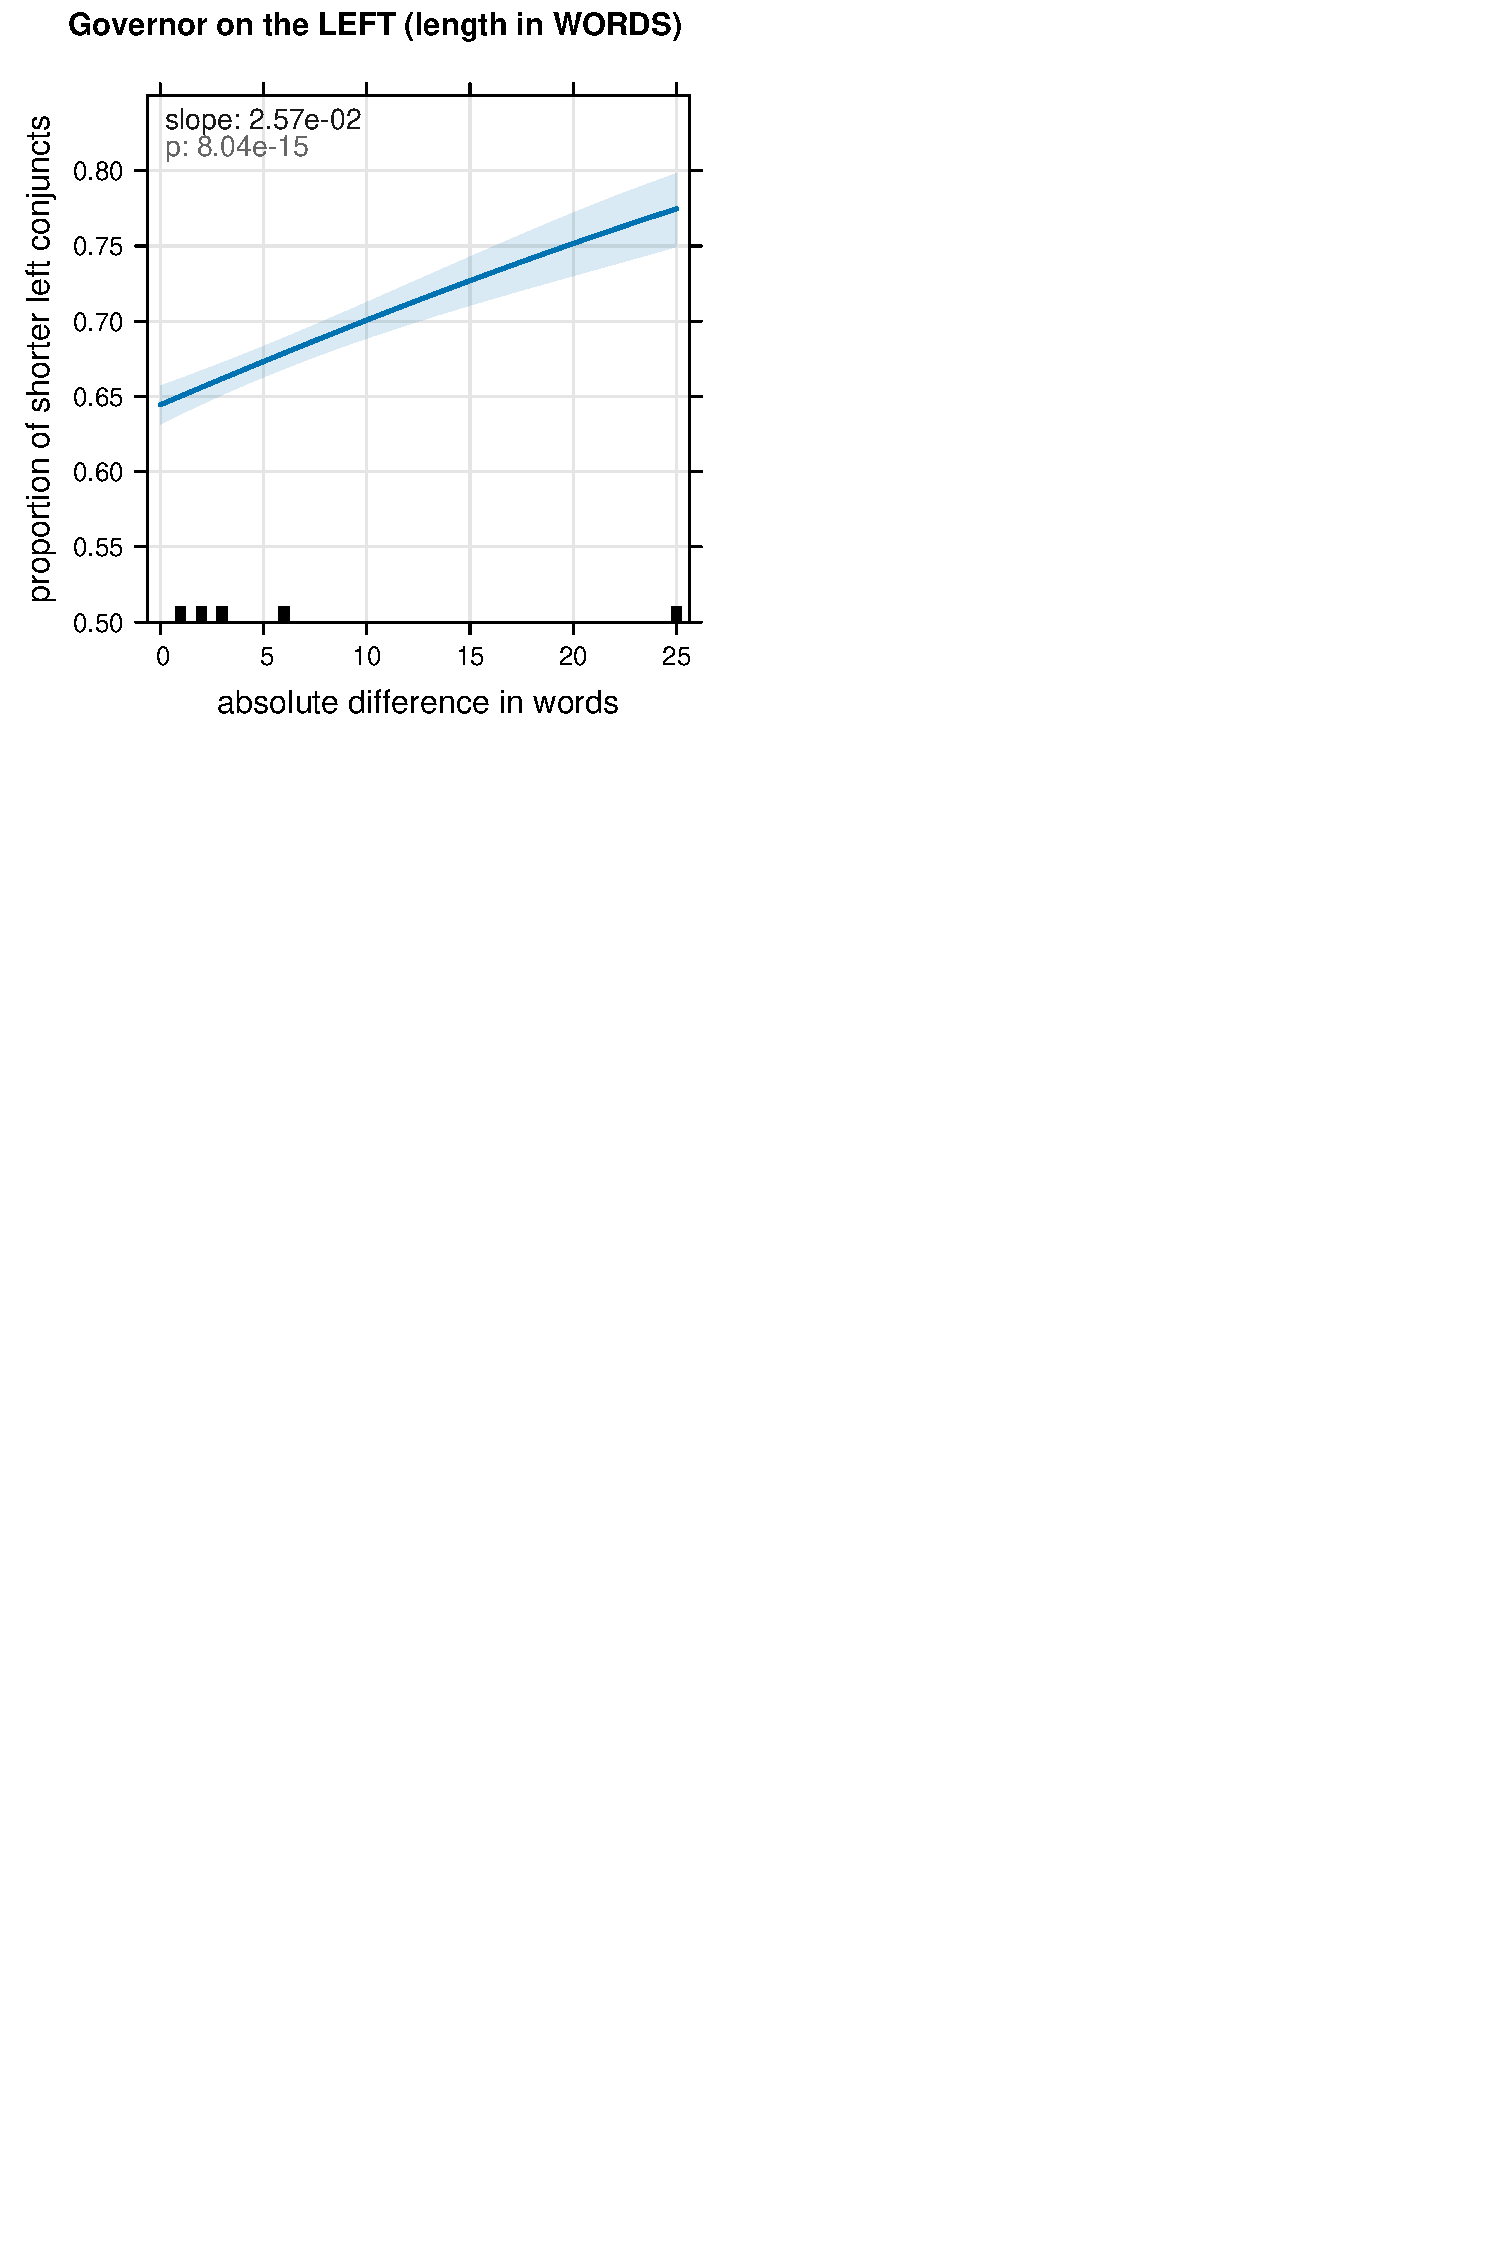
\includegraphics[scale=0.35]{inputs/ptb-L.pdf}
    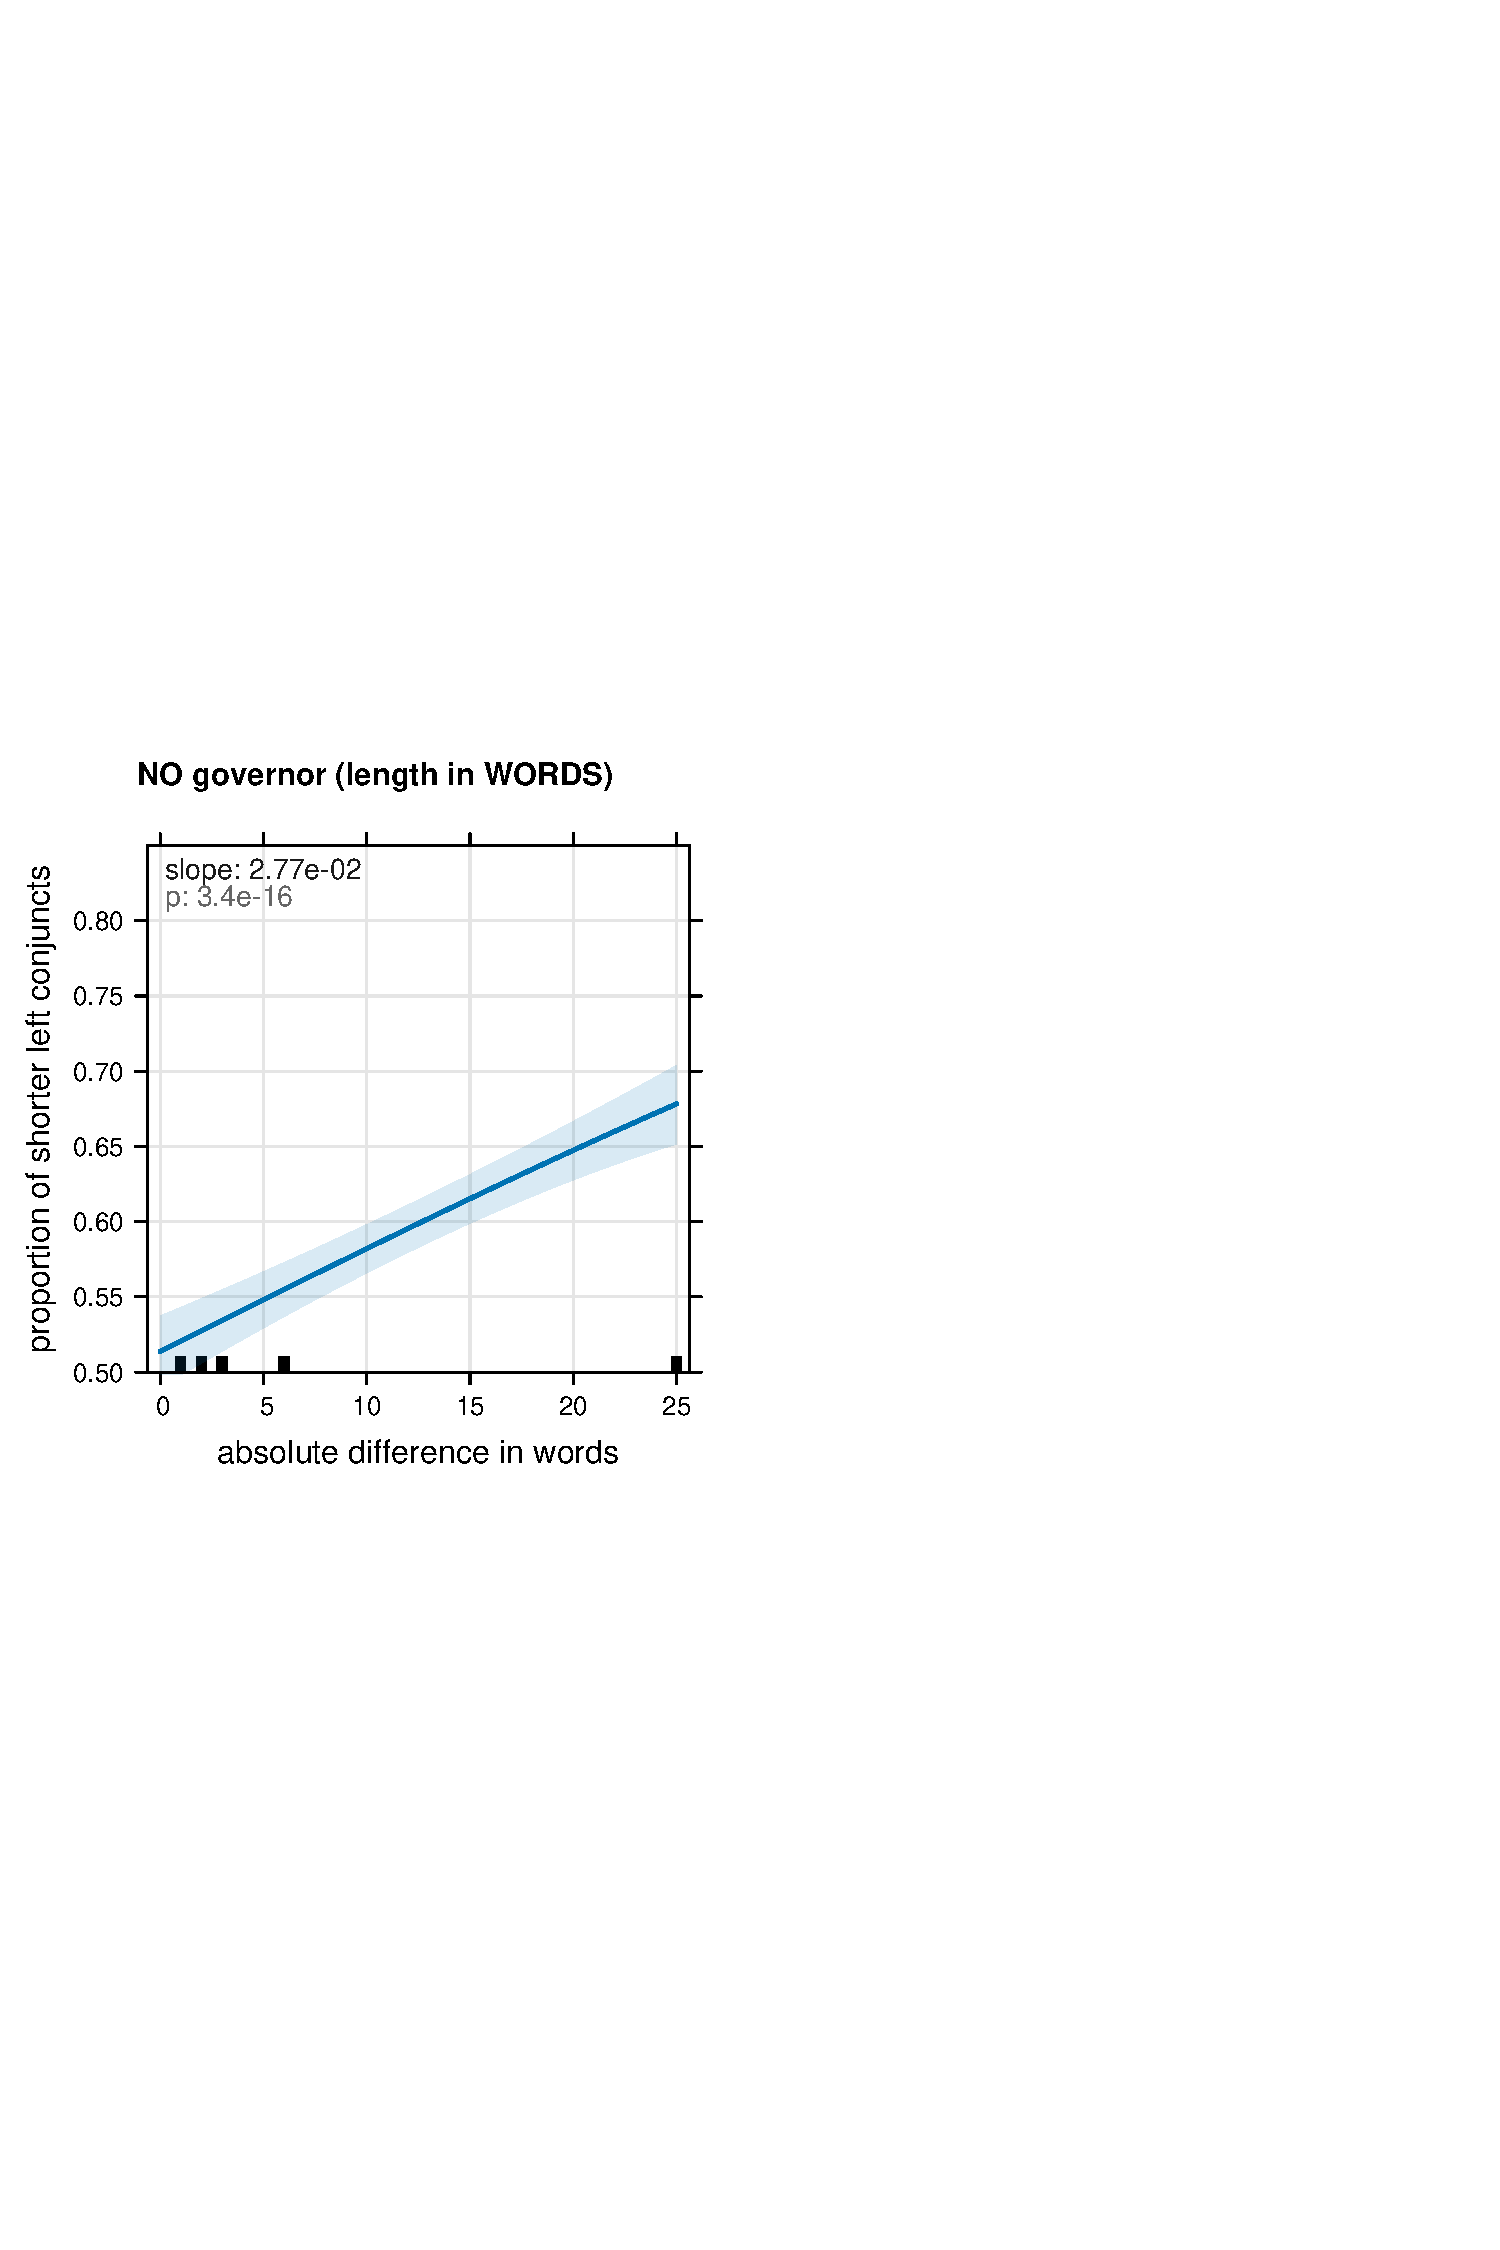
\includegraphics[scale=0.35]{inputs/ptb-0.pdf}
    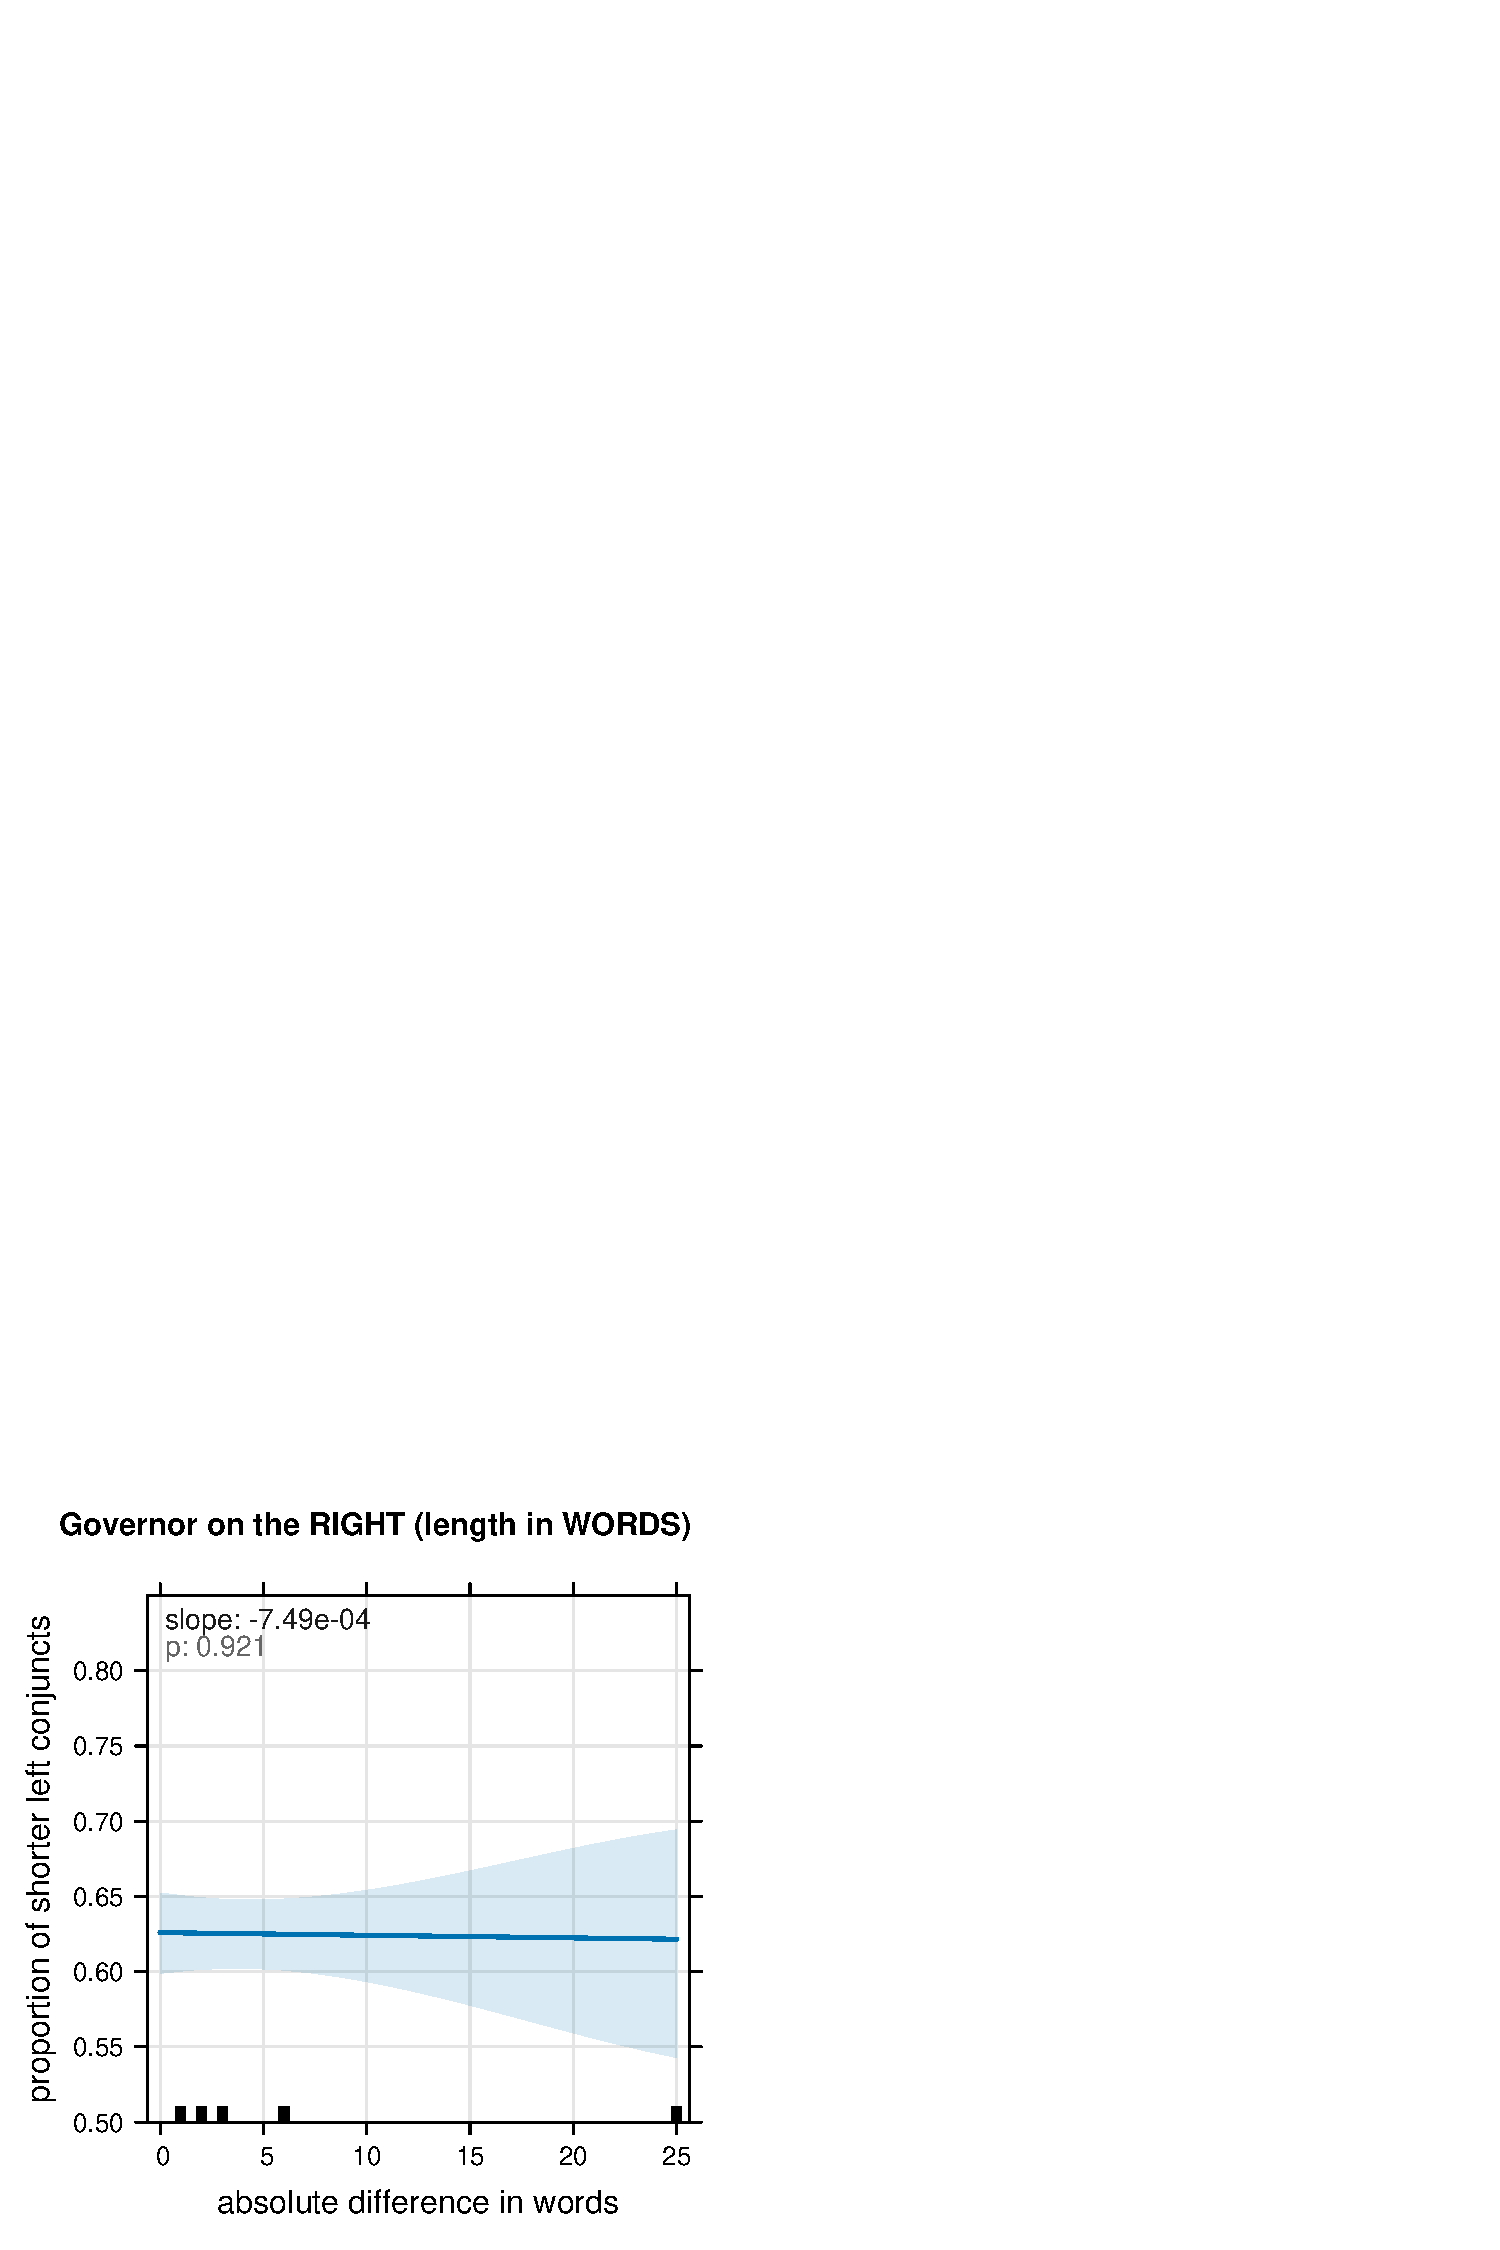
\includegraphics[scale=0.35]{inputs/ptb-R.pdf}
    \caption{Modelled proportions of coordinations with left conjuncts shorter depending on difference in conjunct lengths from \cite{prz:woz:23}}\label{fig:pw23-results}
\end{figure}

Those results are compatible with the predictions of the symmetric annotation styles: the Prague one, assuming DLM working at the level of usage and the London one, assuming also DLM at the level of grammar. An example of DLM in grammar was given in Section \ref{sec:dlm}, but it was not described how it could present itself in coordinations. As was mentioned previously, English is a mostly head-initial language, which in  coordinations means that the governor is usually on the left. When the governor is in fact on the left, the dependencies are shortest when the shorter conjunct is also on the left. There is therefore a grammatical pressure to always put shorter conjuncts on the left, because it should usually lead to shorter dependencies in total. This means that when the coordination has no governor and there is no immediate pressure to order the conjuncts in any way, the shorter conjunct still may be placed on the left, because there is a grammatical pressure to do so.  However as \cite{prz:woz:23} point out, this pressure may be reduced when the length differences between conjuncts are noticably bigger, because then the DLM effect at the level of usage is stronger. 

\cite{pbg2023} have already conducted a replication study of this research. The aim was to see whether the conclusions drawn in the original study hold up when the data come from a bigger and more diverse corpus. The results are presented in Figure \ref{fig:pbg24-results} -- slightly different from what was found in the original study, but they sharpened the original conlusions. In the bigger dataset the coordinations with the governor on the left and without a governor behave the same -- with growing length differences between conjuncts grows also the proportion of shorter left conjuncts. The difference is that, with the governor on the right, proportion of coordinations with the shorter conjunct on the left decreases with the growing length difference. 

\begin{figure}[H]
    \centering
    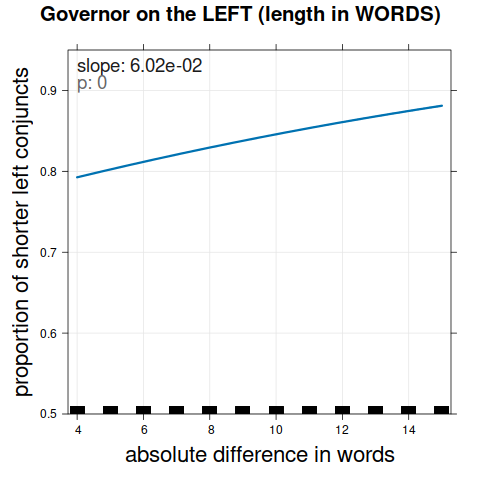
\includegraphics[scale=0.27]{inputs/coca-L.png}
    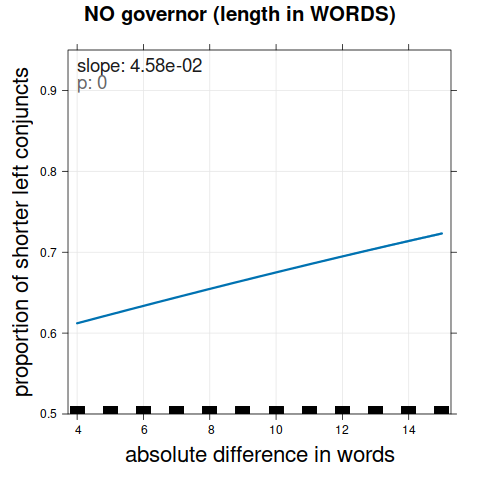
\includegraphics[scale=0.27]{inputs/coca-0.png}
    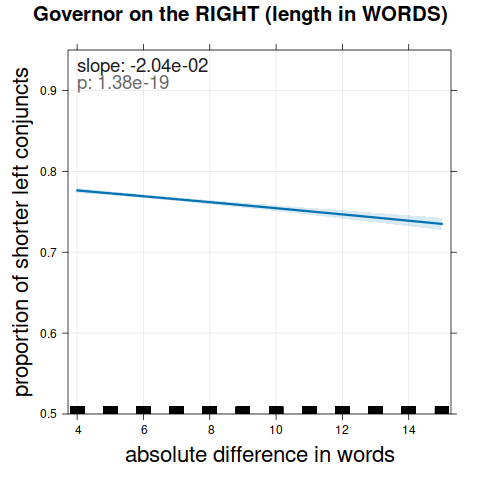
\includegraphics[scale=0.27]{inputs/coca-R.png}
    \caption{Modelled proportions of coordinations with left conjuncts shorter depending on difference in conjunct lengths from \cite{pbg2023}}\label{fig:pbg24-results}
\end{figure}

Those results point to only one of the annotation styles, namely the London one. Within this style, dependencies are minimised when the shorter conjunct is placed closer to the governor if there is one. If the coordination has no governor, neither placement should be preferred, unless DLM at the level of grammar is taken into account -- then the shorter conjunct should be preferred on the left, since that usually helps minimise the dependencies.

\cite{prz:woz:23} conducted their study on a relatively small, but manually annotated corpus. \cite{pbg2023} replicated that study on a larger, but automatically annotated corpus. This automatic annotation resulted in a poor quality of data -- after evaluating the coordinations extracted for analysis, they found only 50.1\% of their sample to be correctly extracted. This study attempts the replication again, with the same larger corpus but aiming to improve the quality of the automatic annotation.

\section{Universal Dependencies}\label{sec:ud}
% theres a project that tries to maybe sort of unify all those ideas for dependency annotation? they want it to be universal, heres how they decided to do it and heres other things about it that will be relevant later (criterion for choosing heads). its been perceived as pretty universal, its used a lot, everywhere almost. there are also enhanced universal depencies, they should be mentioned somewhere although they are not very related to what is described here

% why it was created
As seen in Section \ref{sec:coord annotations}, there are many ideas on the structure of coordination. Universal Dependencies (UD, henceforth) is a project focused on formulating guidelines for creating dependency annotation, that would suit as many languages as possible, while maintaining the possibility to represent phenomena specific to any given language. The guidelines outline how one should deal with word segmentation, part-of-speech tagging, assigning morphological features and creating an appropriate dependency structure for a sentence. 

% criteria for choosing dependency heads
Here, the most relevant part of the project are the rules for creating a dependency structure. In the first version of UD \citep{ud1}, three of them were specified: 
\begin{enumerate}
    \item dependency relations appear between content words,
    \item function words are attached to the content words which they describe,
    \item punctuation marks are attached to the head of the phrase or clause in which they appear.
\end{enumerate}
Content words chosen here for dependency heads can otherwise be called ``lexical'' or ``semantic'' centres, whereas function words serve mostly a syntactic purpose in a sentence. In sentence (\ref{ex:ud eng tree}), the word \textsl{participate} carries the meaning, therefore it is the content word and the root of the sentence. The word \textsl{will} is a function word and is attached to the content word.

\begin{adjustwidth}{-40pt}{-40pt}
\vspace{2ex}
\begin{tabular}{l r}
\begin{minipage}[t][12ex][b]{40ex}
\begin{exe}
    \ex\label{ex:ud eng tree}
    \begin{dependency}[baseline=-\the\dimexpr\fontdimen22\textfont2\relax]
        \begin{deptext}
            Ivan\&will\&participate\&in the show\&.\\
        \end{deptext}
        \deproot{3}{root}
        \depedge{3}{1}{nsubj}
        \depedge{3}{2}{aux}
        \depedge{3}{4}{nmod}
        \depedge{3}{5}{punct}
    \end{dependency}
\end{exe}
\end{minipage}
&
\hspace{20pt}
\begin{minipage}[t][12ex][b]{40ex}
\begin{exe}
    \ex\label{ex:ud fr tree}
    \begin{dependency}[baseline=-\the\dimexpr\fontdimen22\textfont2\relax]
        \begin{deptext}
            Ivan\&participera\&au spectacle\&.\\
        \end{deptext}
        \deproot{2}{root}
        \depedge{2}{1}{nsubj}
        \depedge{2}{3}{nmod}
        \depedge{2}{4}{punct}
    \end{dependency}
\end{exe}
\end{minipage}
\end{tabular}
\vspace{2ex}
\end{adjustwidth}

The reasoning behind setting those criteria is that it increases the chance of finding similar tree structures in different languages, for example when comparing sentences between English and French, which is morphologically richer. (\ref{ex:ud fr tree}) is a tree for the French translation of the sentence in (\ref{ex:ud eng tree}). Even though the French sentence does not have an auxiliary word to mark the future tense, the structures of those sentences are almost identical, which would not be possible if UD chose to make functional words governors of content words.

\section{Surface-syntactic Universal Dependencies}\label{sec:sud}
% there was another idea for universal dependency annotation scheme, they want to be universal too, but in a different way, more syntactic but only on the surface. thats why they called themselves surface syntactic universal dependencies. they maybe slightly disagreed with some decisions made in UD so they made their own version. heres how they differ in ways that important for me
Surface-syntactic Universal Dependencies (SUD, henceforth) is another example of a project aiming to create a set of universal guidelines for dependency annotation. \cite{gerdes-etal-2018-sud} describe it as ``near-isomorphic to UD'' and propose a set of conversion rules between the schemes. Most of the SUD annotation guidelines are the same as in UD, the most prominent difference is the change in choosing dependency heads, from content words to function words. This section covers the relevant differences between the schemes and how those are beneficial for research described in this work.

\subsection{Criteria for choosing heads of dependencies}\label{sec:sud criteria}
Instead of favouring content words, SUD uses the distributional criteria for choosing dependency heads, which means that ``the surface syntactic head determines the distribution of the unit'' \citep{gerdes-etal-2018-sud}. It can be tested by checking which of the words within a dependency behaves in sentences similarly to the way the whole unit does, so which of the words can be replaced by the unit and \textsl{vice versa}. The example sentence the authors use to explain their criteria is \textsl{The little boy talked to Mary}. There is a dependency between words \textsl{little} and \textsl{boy}, and sentences in (\ref{ex:distribution boy}) and (\ref{ex:distribution little}) show why the head of this dependency is the word \textsl{boy}. In (\ref{ex:distribution boy}a) the word \textsl{boy} can be replaced by the unit \textsl{little boy}, as shown in (\ref{ex:distribution boy}b), and the sentence is still grammatical. 

\begin{exe}
    \ex
    \label{ex:distribution boy}
    \begin{xlist}
        \ex[] {I saw a \textbf{boy}.}
        \ex[] {I saw a \textbf{little boy}.}
    \end{xlist}
\end{exe}

The same is not the case for the word \textsl{little}. Trying to replace that word with the whole unit in (\ref{ex:distribution little}a) results in an ungrammatical sentence in (\ref{ex:distribution little}b). Sentences (\ref{ex:distribution little}c--d) show that replacement in the other way is not possible either, therefore the word \textsl{little} cannot be the head of this dependency.

\begin{exe}
    \ex
    \label{ex:distribution little}
	\begin{xlist}
    		\ex[] {The boy was \textbf{little}.}
    		\ex[*] {The boy was \textbf{little boy}.}
    		\ex[] {I found the \textbf{little boy}.}
    		\ex[*] {I found the \textbf{little}.}
    \end{xlist}
\end{exe}

It is not always possible to test both of the words within a dependency, but in such cases showing that one of the words does not commute with the whole unit is enough to decide it is not the head, therefore the other one must be. As shown in \cite{gerdes-etal-2018-sud}, that is exactly the case with the words \textsl{to Mary} -- it is impossible to see how the word \textsl{to} behaves on its own, as it needs a noun or a verb, but the sentences in (\ref{ex:distribution Mary}) show that \textsl{Mary} does not have the same distribution as those two words together.

\begin{exe}
    \ex
    \label{ex:distribution Mary}
    \begin{xlist}
    		\ex[] {I saw \textbf{Mary}.}
    		\ex[*] {I saw \textbf{to Mary}.}
    		\ex[] {I talked \textbf{to Mary}.}
    		\ex[*] {I talked \textbf{Mary}.}
    \end{xlist}
\end{exe}

This key difference between UD and SUD has crucial consequences for extracting the exact length of conjuncts in a coordinate structure, which is an integral part of this work. As \cite{prz:woz:23} mention, the UD scheme is not ideal for coordination analysis, as it is not clear which dependencies are shared by the conjuncts and which are private. This is illustrated by the sentences in (\ref{ex:drink-and-drive}) and (\ref{ex:rapidly-expand}).

\begin{adjustwidth}{-40pt}{-40pt}
    \vspace{4ex}
    \begin{tabular}{lr}
    \begin{minipage}[t][12ex][b]{40ex}
    \begin{exe}
    \ex\label{ex:drink-and-drive}
    \begin{dependency}[baseline=-\the\dimexpr\fontdimen22\textfont2\relax]
        \begin{deptext}
            Never\& drink\& and\& drive\& .\\
        \end{deptext}
        \deproot{2}{root}
        \depedge{2}{1}{advmod}
        \depedge{2}{4}{conj}
        \depedge{4}{3}{cc}
        \depedge{2}{5}{punct}
    \end{dependency}
    \end{exe}
    \end{minipage}
    &
    \begin{minipage}[t][12ex][b]{40ex}
    \begin{exe}
        \ex\label{ex:rapidly-expand}
        \begin{dependency}[baseline=-\the\dimexpr\fontdimen22\textfont2\relax]
            \begin{deptext}
                 Rapidly\& expanded\& and\& blew\& up\&.\\
            \end{deptext} 
            \depedge{2}{1}{advmod} 
            \depedge{2}{6}{punct}
            \deproot{2}{root} 
            \depedge[edge height=2ex]{4}{3}{cc} 
            \depedge{2}{4}{conj}  
            \depedge[edge height=4ex]{4}{5}{compound:prt}
        \end{dependency}
    \end{exe}
    \end{minipage}
    \end{tabular}
\end{adjustwidth}

In (\ref{ex:drink-and-drive}) the coordinated words are \textsl{drink} and \textsl{drive}, the word \textsl{never} is attached to the first conjunct and even though English speakers reading this sentence know that it applies to the whole coordination, it is not obvious from the structure of the sentence. The structure in (\ref{ex:rapidly-expand}) is similar, but this time the word \textsl{rapidly} applies only to the first conjunct. In both of those sentences knowledge of the real world is required to accurately determine whether the dependency is shared by the whole coordination (as in (\ref{ex:drink-and-drive})) or private to the first conjunct (as in (\ref{ex:rapidly-expand})). Because of this ambiguity, it is difficult to construct accurate heuristics for determining the extent of each conjunct in a coordination. This issue appears in both UD and SUD, however the following examples show that some of the ambiguities present in UD can be resolved in SUD.

% why is that important for me -- give an example of a sentence with a coordination where one of the conjuncts has an auxiliary dependency, which would be troubling to decipher automatically using UD, but not SUD
Based on heuristics used by \cite{pbg2023}, the tree in (\ref{ex:UD magma}) would give a coordination with conjuncts \textsl{reach the surface} and \textsl{cools at depth}. This is, because the head of the left conjunct, \textsl{reach}, has on its left side dependencies labeled \texttt{nsubj}, \texttt{advmod} and \texttt{aux}, but the head of the right conjunct, \textsl{cools}, does not have any of those dependencies. Therefore all of those dependencies are predicted to be shared by both conjuncts. The correct parse of this sentence gives a coordination with conjuncts \textsl{does not reach the surface} and \textsl{cools at depth}, so the dependencies \textsl{This magma often} should not be shared, but private to the first conjunct. 

\begin{adjustwidth}{-20pt}{20pt}
\begin{exe}
    \ex\label{ex:UD magma}
    \begin{dependency}[hide label, baseline=-\the\dimexpr\fontdimen22\textfont2\relax]
        \begin{deptext}
            This\& magma\& often\& does\& not\& reach\& the\& surface\& but\& cools\& at\& depth.\footnotemark\\
        \end{deptext}
    \depedge{2}{1}{det} 
    \depedge[show label]{6}{2}{nsubj} 
    \depedge[show label]{6}{3}{advmod} 
    \depedge[show label]{6}{4}{aux} 
    \depedge[show label]{6}{5}{advmod} 
    \deproot[show label, edge height=3cm]{6}{root} 
    \depedge{8}{7}{det} 
    \depedge{6}{8}{obj} 
    \depedge[show label]{10}{9}{cc} 
    \depedge[show label, edge height=2cm, theme=night]{6}{10}{conj} 
    \depedge{12}{11}{case} 
    \depedge[show label]{10}{12}{obl} 
\end{dependency}
\end{exe}
\footnotetext{Sentence \texttt{w01031015} from the \texttt{UD\_English-PUD} corpus \citep{pud}.}
\end{adjustwidth}

\begin{adjustwidth}{-20pt}{20pt}
\begin{exe}
\ex\label{ex:UD ballet}
\begin{dependency}[hide label, baseline=-\the\dimexpr\fontdimen22\textfont2\relax]
    \begin{deptext}
        Ballet\& shoes\& should\& be\& snug,\& but\& not\& so\& tight\& they\& cut\& off\& blood\& flow.\footnotemark\\
    \end{deptext}
    \deproot[show label, edge height=3cm]{5}{root}
    \depedge[show label]{5}{2}{nsubj}
    \depedge{2}{1}{compound}
    \depedge[show label]{5}{3}{aux}
    \depedge[show label]{5}{4}{cop}
    \depedge[show label, theme=night]{5}{9}{conj}
    \depedge[show label]{9}{6}{cc}
    \depedge[show label]{9}{7}{advmod}
    \depedge[show label]{9}{8}{advmod}
    \depedge[show label]{9}{11}{advcl}
    \depedge{11}{10}{nsubj}
    \depedge{11}{12}{compound:prt}
    \depedge[edge height=1.5cm]{11}{14}{obj}
    \depedge{14}{13}{compound}
\end{dependency}
\end{exe}
\footnotetext{Sentence \texttt{GUM\_whow\_ballet-14} from the \texttt{UD\_English-GUM} corpus \citep{Zeldes2017}.}
\end{adjustwidth}

Modifying the heuristics, so that they fit this example, for instance by saying that \texttt{aux} dependencies should always be included in the left conjunct, would on the other hand mean that sentences such as in (\ref{ex:UD ballet}) would have incorrect extracted coordinations. In this example the correct coordinate structure has conjuncts \textsl{snug} and \textsl{not so tight they cut off blood flow}, but if the algorithm included the \texttt{aux} dependency in the first conjunct (as would be required in (\ref{ex:UD magma})), the result would be conjuncts \textsl{should be snug} and \textsl{not so tight they cut off blood flow}.

This however is not an issue when using the SUD scheme. As shown in (\ref{ex:SUD magma}), the words \textsl{does not} cannot be dependencies of the whole coordination, because the word \textsl{does} is the head of the left conjunct and the word \textsl{not} is one of its dependencies on the right and thus is always included in the conjunct. Changing the annotation scheme to SUD does not affect the sentence in (\ref{ex:UD ballet}) -- the word \textsl{snug} has to be the whole left conjunct, because it also does not have any dependencies in this annotation scheme.

\begin{adjustwidth}{-20pt}{20pt}
\begin{exe}
\ex\label{ex:SUD magma}
\begin{dependency}[hide label, baseline=-\the\dimexpr\fontdimen22\textfont2\relax]
	\begin{deptext}
		This\& magma\& often\& does\& not\& reach\& the\& surface\& but\& cools\& at\& depth.\footnotemark\\
	\end{deptext} 
	\depedge{2}{1}{det} 
	\depedge[show label]{4}{2}{subj} 
	\depedge[show label]{4}{3}{mod} 
	\deproot[show label, edge height=2cm]{4}{root} 
	\depedge{4}{5}{mod} 
	\depedge{4}{6}{comp:aux} 
	\depedge{8}{7}{det} 
	\depedge{6}{8}{comp:obj} 
	\depedge[show label]{10}{9}{cc} 
	\depedge[show label, edge height=1.5cm, theme=night]{4}{10}{conj} 
	\depedge[show label]{10}{11}{udep} 
	\depedge{11}{12}{comp:obj} 
\end{dependency}
\end{exe}
\footnotetext{Sentence \texttt{w01031015} from the \texttt{SUD\_English-PUD}.}
\end{adjustwidth}

\begin{adjustwidth}{-20pt}{20pt}
\begin{exe}
    \ex\label{ex:SUD ballet}
    \begin{dependency}[hide label, baseline=-\the\dimexpr\fontdimen22\textfont2\relax]
        \begin{deptext}
            Ballet\& shoes\& should\& be\& snug,\& but\& not\& so\& tight\& they\& cut\& off\& blood\& flow.\footnotemark\\
        \end{deptext}
    \deproot{3}{root}
    \depedge{3}{2}{subj}
    \depedge{2}{1}{compound}
    \depedge{3}{4}{comp:aux}
    \depedge{4}{5}{comp:pred}
    \depedge[show label, theme=night]{5}{9}{conj}
    \depedge[show label]{9}{6}{cc}
    \depedge[show label]{9}{7}{mod}
    \depedge[show label]{9}{8}{mod}
    \depedge[show label]{9}{11}{mod}
    \depedge{11}{10}{subj}
    \depedge{11}{12}{compound@prt}
    \depedge{11}{14}{comp:obj}
    \depedge{14}{13}{compound}
    \end{dependency}
\end{exe}
\footnotetext{Sentence \texttt{GUM\_whow\_ballet-14} from the \texttt{SUD\_English-GUM} corpus.}
\end{adjustwidth}

Therefore, the focus on syntax in SUD makes it a better fit for coordination analysis.

\subsection{Explicit information about shared dependencies}\label{sec:shared-deps}
Besides the structural advantages that SUD has over UD when it comes to analysing coordination, there is one additional feature that is added in SUD treebanks that helps find the extent of conjuncts. 

While UD corpora are often created specifially for the purpose of participating in the UD project or converted with manual corrections from different dependency annotations, the SUD corpora are mostly converted automatically from UD. There are a few French treebanks, as well as treebanks for Beja, Zaar, Chinese and Naija, that are natively made for SUD, but all others are converted from UD using rule-based graph transformation grammars, which are described in more detail in Chapter 3. 

As was mentioned in Section \ref{sec:coord annotations}, UD uses the Bouquet approach to annotating coordination, while SUD uses the Chain one. This means that in the conversion process, some information about the privacy status of a dependency of the coordination can be lost. This is visible in the coordination presented in the sentence \textsl{I just sat in there for like an hour and a half straight and studied}.\footnote{Sentence \texttt{GUM\_vlog\_studying-27} from the GUM corpus \citep{Zeldes2017}.} As the UD annotation in (\ref{ex:UD 1,5h straight}) shows, the word \textsl{straight} is shared by the whole structure. This is not structurally visible in the SUD version in (\ref{ex:SUD 1,5h straight}), where the \texttt{mod} dependency for the word \textsl{straight} is attached to the last conjunct. 

\begin{adjustwidth}{-50pt}{-50pt}
\vspace{2ex}
\centering
\begin{tabular}{lr}
\begin{minipage}[t][9ex][b]{8cm}
\begin{exe}
    \ex\label{ex:UD 1,5h straight}
    \begin{dependency}[baseline=2.8ex]
        \begin{deptext}
            an\&hour\&and\&a\&half\&straight\\
            \&\&\&\&\&\footnotesize\textsf{upos=ADV}\\
            \&\&\&\&\&\footnotesize\textsf{lemma=straight}\\
            \&\&\&\&\&\footnotesize\textsf{Degree=Pos}\\
        \end{deptext}
        \depedge[edge height=6ex]{2}{5}{conj}
        \depedge[edge height=3ex]{5}{3}{cc}
        \depedge[edge height=8ex]{2}{6}{advmod}
    \end{dependency}
\end{exe}
\end{minipage}
&
\begin{minipage}[t][8.8ex][b]{8cm}
\begin{exe}
    \ex\label{ex:SUD 1,5h straight}
    \begin{dependency}[baseline=3.8ex]
        \begin{deptext}
            an\&hour\&and\&a\&half\&straight\\
            \&\&\&\&\&\footnotesize\textsf{upos=ADV}\\
            \&\&\&\&\&\footnotesize\textsf{lemma=straight}\\
            \&\&\&\&\&\footnotesize\textsf{Degree=Pos}\\
            \&\&\&\&\&\footnotesize\textsf{Shared=Yes}\\
        \end{deptext}
        \depedge[edge height=6ex]{2}{5}{conj}
        \depedge[edge height=3ex]{5}{3}{cc}
        \depedge{5}{6}{mod}
    \end{dependency}
\end{exe}
\end{minipage}
\end{tabular}
\end{adjustwidth}

So as not to lose this information while converting the annotation scheme, feature \textsf{Shared=Yes} is added. Similarly, in coordinations where a dependent is attached to the right conjunct in the UD scheme (therefore private to the right conjuct), during the conversion to SUD the feature \textsf{Shared=No} is added.

\subsection{Learnability of dependency schemes}\label{sec:learnability}
% in pbg23 they tried to use ud but failed (50.1%)
The current study is another replication of \cite{prz:woz:23}. As was pointed out in Chapter \ref{ch:introduction}, \cite{pbg2023} have conducted a similar analysis on the COCA corpus annotated automatically in the UD scheme. After evaluating the automatically annotated data they found only 50.1\% of the coordinations in the evaluation sample to be correctly extracted from the corpus. Reasons for such an outcome can be twofold: the issues lie either within the parsing accuracy or within the script for extracting coordinations from dependency trees. 

Issues within the script have been addressed to some extent in Section \ref{sec:sud criteria} -- heuristics for finding conjunct extents are easier to develop within a function-word focused annotation scheme. As for the parsing performance, there are studies showing that the UD scheme is harder to parse. \cite{rehbein-etal-2017-universal} show that choosing content words rather than function words for dependency heads increases arc direction entropy (a measure describing how consistent dependency directions in a given treebank are), which then lowers parsing accuracy. In another study, \cite{kohita-etal-2017-multilingual} converted UD trees into ones with function heads, rather than content heads. They then used the converted trees for training parsers and parsed 19 treebanks using both UD and converted models. After parsing, the results from the converted models were converted back to UD and for most of the languages (11 out of 19) those results had better scores. 

The criterion for choosing dependency heads may not be the only structural advantage that SUD has over UD in terms of parsing. As \cite{gerdes-etal-2018-sud} demonstrate, the Chain approach to annotating coordination, that is used in SUD, minimises the dependency lengths compared to the Bouquet approach used in UD. This may be beneficial for parsing accuracy, as parsers tend to perform better when working with shorter dependencies \citep{nilsson-etal-2006-graph, eisner-smith-2005-parsing}. 
% could add here about shorter dependencies in SUD than UD in general, citing typometrics.elizia.net, but idk how to do that
% As can be observed in [typometrics], SUD has overall shorter dependencies than UD, therefore whole SUD structures might prove to be easier to parse than UD ones and possibly yield better results at the evaluation stage. 

In the studies cited above the comparison was between UD and a scheme that differed from UD only in some particular aspect, not a new, comprehensive scheme. \cite{tuo:prz:lac:21}, however, compared UD to SUD, which matters because, as they say, ``any realistic annotation schema which employs a more ‘syntactic’ approach to headedness than UD will also differ from UD in the repertoire and distribution of dependency labels, and will also take into account the intrinsic linguistic interaction between various constructions''. They trained five parsers, two of which were transition-based and three graph-based, using 21 corpora representing 18 languages. While transition-based parsers seemed to perform similarly on both annotation schemes, the graph-based ones preferred SUD. As for attachment scores for the English corpus tested in this experiment (GUM), all of the parsers scored higher with the SUD annotation. The parser utilised in the current study, Stanza, is graph-based and the language of the texts it annotates is English, therefore SUD might be the better choice for the annotation scheme for this data. 

%\section{Summary}
% to summarise, you can try to see the syntactic structure of a sentence in different ways, i.e. constituency or dependency (any others?). dependency ones are important here, because i use those approaches in the current study. i use a parser to add syntactic annotation to a large corpus. the parser im using is said to work better with SUD rather than UD, so thats the scheme im choosing. the next chapters describe the exact ways in which this syntactic annotation is added and how i later extract the information that i need.

\bibliography{bibliography}

\end{document}
